% !TeX spellcheck = fa
\documentclass[a4paper,12pt]{report}

\usepackage{color}
\usepackage{float}
\usepackage{babel}
\usepackage{fourier}
\usepackage{amsmath}
%% \usepackage{dirtree} %to show tree view directories.
\usepackage{caption}
\usepackage{nomencl}
\usepackage{verbatim}
\usepackage{fancyhdr}
\usepackage{graphicx}
\usepackage{geometry}
\usepackage{outlines}
\usepackage{enumitem}
\usepackage{fancyvrb}
\usepackage{listings}
\usepackage{makecell}
\usepackage{tabularx} % for custom width table
\usepackage{subcaption}
\usepackage{datenumber}
\usepackage{indentfirst}
\usepackage{lstautogobble}
\usepackage[table]{xcolor}
\usepackage[utf8] {inputenc}
\usepackage[space]{grffile}
\usepackage[final]{pdfpages}
\usepackage[datesep=.,calc,showdow]{datetime2}
\usepackage{accsupp}

%% \usepackage[perpage]{footmisc}
\usepackage[breakable]{tcolorbox}
\tcbuselibrary{breakable, skins}
\usepackage[Bjornstrup]{fncychap}
%Options: Sonny, Lenny, Glenn, Conny, Rejne, Bjarne, Bjornstrup
\usepackage[colorlinks,linkcolor=blue,citecolor=red,urlcolor=blue]{hyperref}

%% \usepackage[style=long,toc,xindy]{glossaries}
%% \usepackage[symbols,nogroupskip,sort=standard]{glossaries-extra}

\usepackage[fontsize={12,18}]{xepersian}

\DTMsetup{useregional}
% -------------- tcolorbox -------------
\tcbset{
	enhanced,
	colback=cyan!5!white,
	boxrule=0.1pt,
	colframe=cyan!75!black,
	fonttitle=\bfseries,
	width=0.9\linewidth
}

% ------------- font setup -------------
% ------------- xepersian --------------
%% \settextfont{Microsoft Sans Serif}
\settextfont		{Yas}
\setmathdigitfont	{Yas}
\setlatintextfont	{Arial}
\defpersianfont\XBT	[Scale=1.1]{XB Titre}
\deflatinfont\FS	[Scale=16]{Far.Symbol8}
\deflatinfont\TNR	[Scale=1]{Arial}
\deflatinfont\CNSLS	[Scale=1]{Consolas}

% --------------   xcolor  -------------
\definecolor{ao}{rgb}			{0.00, 0.50, 0.00}
\definecolor{codeGreen}{rgb}	{0.00, 0.50, 0.50}
\definecolor{lavendergray}{rgb}	{0.87, 0.86, 0.92}
\definecolor{mint}{rgb}			{0.24, 0.71, 0.54}
\definecolor{aliceblue}{rgb}	{0.94, 0.97, 1.00}
\definecolor{commentGreen}{rgb}	{0.13, 0.65, 0.47}
\definecolor{steelBlue}{rgb}	{0.00, 0.00, 0.50}
\definecolor{stringGreen}{rgb}	{0.00, 0.50, 0.00}
\definecolor{rowBlue}{rgb}		{0.48, 0.81, 0.87}

% ---------  page header setup ---------
% --------------  fancyhdr -------------
\pagestyle{fancy}

\cfoot{\thepage}
\rhead{\thepage }
\renewcommand{\headrulewidth}{0.4pt}

%% new commands.
\newcommand{\lrm}[1]{\textcolor{steelBlue}{\lr{\texttt{#1}}}}
\newcommand{\qt}[1]{''#1``}
\newcommand{\LTRqt}[1]{``#1''}

%% tabular borders color
\arrayrulecolor{gray}

\renewcommand{\bibname}{مراجع}
% \newglossaryentry{dot-product}{name={dot product},description={aaa}}
% \makeglossaries
\makenomenclature
\renewcommand{\nomname}{فهرست علائم}
\nomenclature{$\bullet$}{bullet}

%% ugly chapter style for chapters :D
% --------- chapter renew command -------------
\newcommand{\opchapter}[1]{\newpage%
	\topskip0pt%
	\vspace*{\fill}%
	\addtocounter{chapter}{1}%
	\begin{center}%
		\textbf{\huge{\color{gray}{فصل \thechapter \\[1cm] \uppercase{#1}}}}%
	\end{center}%
	\vspace*{\fill}%
	\newpage%
	\textbf{\Large{\thechapter. #1}}%
	\addcontentsline{toc}{chapter}{#1}%
}

\geometry{
	a4paper,
	top		= 35mm,
	right	= 35mm,
	bottom	= 25mm,
	left	= 25mm,
}

\newcommand{\AlterText}{%
	\BeginAccSupp{method=pdfstringdef,unicode,ActualText={y}}%
	x%
	\EndAccSupp{}%
}

\renewcommand{\today}{۲۷ مهر ۱۴۰۲}
\renewcommand{\DTMtoday}{19 October, 2023}


\begin{document}
	\definecolor{jkey}{rgb}{0.13, 0.55, 0.13}
	\definecolor{jnumber}{rgb}{0.78, 0.39, 0.0}

	\lstdefinelanguage{graphql}{
		keywords={ID, Boolean, Int, Float, Command, Field, Query, State, Boundary, input, LatestStatus, String, User, Session, DeviceType},
		keywordstyle=\color{blue}\bfseries,
		identifierstyle=\color{black},
		sensitive=false,
		comment=[l]{//},
		morecomment=[s]{/*}{*/},
		morestring=[b]',
		morestring=[b]"
	}

	\lstdefinelanguage{qml}{
		keywords={id, typeof, new, true, false, catch, function, return, null, catch, switch, var, if, in, while, do, else, case, break},
		keywordstyle=\color{blue}\bfseries,
		ndkeywords={property, float, int, bool, class, export, boolean, throw, implements, import, this},
		ndkeywordstyle=\color{darkgray}\bfseries,
		identifierstyle=\color{black},
		sensitive=false,
		comment=[l]{//},
		morecomment=[s]{/*}{*/},
		morestring=[b]',
		morestring=[b]"
	}

	\lstset{
		frame		=	tb,
		basicstyle	=	\color{steelBlue}\linespread{0.8}\CNSLS,
		columns		=	fullflexible,
		keepspaces	=	false,
		tabsize		=	3,
		autogobble		,
		breaklines	=	true,
		breakatwhitespace=true,
		stringstyle	=	\color{stringGreen},
		commentstyle=	\color{gray},
		keywordstyle=	\color{purple},
		language	=	c++,
		aboveskip	=	3mm,
		belowskip	=	3mm,
		showstringspaces=false,
		columns		=	flexible,
		captionpos	=	b,
		numbers		=	left,
		numbersep	=	5pt,
		numberstyle	=	\color{gray}\linespread{0.8}\ttfamily,
		postbreak	=	\mbox{\textcolor{blue}{$\hookrightarrow$}\space}
	}

	\thispagestyle{empty}
	\begin{center}
		{
			\qquad\FS 3
		}
	\end{center}
	\vspace*{10cm}\newpage\thispagestyle{empty}\vspace*{10cm}\newpage

	\title{
		
\includegraphics[width=0.5\textwidth]{images/quct-logo.pdf}\\[10mm]
		\XBT\normalsize
			پروژهٔ کارشناسی \\[5mm]
			\Large
			سیستم دزدگیر خودرو \\
            \lr{Cardian}
	}
	\author{
		\XBT
		سیّد مرتضیٰ رضوی\\
		\XBT
		دکتر صادقی زاده
	}
	\date{
		\XBT
		\normalsize
		\today
	}

	\pagenumbering{roman}
	\maketitle
	\setcounter{page}{1}
	\tableofcontents
	%\printnomenclature
	\listoffigures
	%\listoftables

	\newpage
	\pagenumbering{arabic}

	\opchapter{
	معرفی
	}\label{chap1}

	\section{
	شرح کلی پروژه
	}\label{sec1:chap1}
	این پروژه در حول پیاده سازی یک سیستم هشدار خودرو یا در اصطلاح دزدگیر خودرو است.

	پروژه شامل دو بخش پیاده سازی سخت‌افزاری دزدگیر و هستهٔ اصلی و پیاده سازی بخش نرم‌افزاری به صورت
	\lr{android application}
	به منظور کنترل بهتر بخش سخت‌افزاری در نظر گرفته شده‌است.

	معمولاً این نوع دستگاه‌ها به منظور فقط کاربرد هشدار دادن استفاده می‌شود، اما از طرفی سهولت استفاده از خودرو نیز مد نظر طراحان این نوع دستگاه قرار دارد.

	دزدگیر‌های خودرو به نوعی از عصر ورود خودروها به بازار آمدند، یک دزدگیر در دو نوع کارخانه و پس از فروش بر روی خودرو متصل می‌شوند.

	در حالت کارخانه عموماً امکانات ساده‌ای مانند هشدار در صورت ضربه و بازکردن درها قرار دارد.

	در نوع دیگر که به صورت جدا و معمولاً به صورت محصول شرکتی مستقل بر روی خودرو متصل می‌شود که امکانات بسیار بیشتری نسبت به انواع کارخانه‌ای دزدگیر دارد.

	این پروژه شامل بخش زیادی از پیاده سازی این امکانات در کنار استفاده از تراشه‌های ارزان قیمت در محصول نهایی است.

	که می‌توان به امکان مکان‌یابی و مشاهدهٔ وضعیت خودرو از طریق
	\lr{application}
	به کاربر نیز اشاره کرد.


	\section{
	اهداف
	}\label{sec2:chap1}
	امروزه دزدگیر خودرو به یک استاندارد و یک وسیله مورد نیاز هر خودرو شخصی بدل شده‌است،
	از طرفی طی چند سال عملکرد‌های دزدگیر خودرو بهبود یافته‌است،‌ تا حدی که در ارسال دستورات
\lr{remote}
	از رمزنگاری و روش‌های پنهان سازی دستورات برای جلوگیری از دزدی و حملات مخرب صورت گرفته است.
	اهداف این پروژه، به طور خلاصه و کلی شامل:
	\begin{itemize}[nosep]
		\item
		پیاده سازی هرچه ارزانتر محصول نهایی، که منوت به استفاده تراشه‌های ارزان قیمت در محصول می شود.
		\item
		ایجاد یک روش و رمزنگاری مناسب سیگنال ارسالی به وسیله
		\lr{remote}.
		\item
		کنترل حدالامکان خودرو با استفاده از
		\lr{application}.
		\item
		و همچنین استفاده از زبان
		\lr{C/C++}
		به منظور
		\lr{performance}
		بالا و کارکرد اجرایی.
	\end{itemize}

		در انتها هدف این پروژه پیاده سازی این دزدگیر با بهترین شرایط کنترل خودرو و ایجاد یک رمزنگاری بهبودیافته نسبت به مابقی سیستم‌ها است، که از طرفی امکان کنترل مناسب خودرو به نسبت دیگر محصولات با قیمت هم سطح را فراهم کند.
	\section{
	پروژه‌های مشابه موجود
	}\label{sec3:chap1}
	از طرفی که یک دزدگیر خودرو به محصولی پر استفاده از زمان پیدایش خودرو مبدل شده است، در نتیجه محصولات زیادی با ويژگی‌های مختلف در این باره معرفی شده‌اند. که در این بخش به معرفی چندی از محصولات پرفروش و پرطرفدار می‌پردازیم.
	\subsection{
		\lr{Viper 5906V}
	}\label{subsec1:sec3:chap1}
	این دزدگیر محصول کمپانی
	\lr{Directed Electronics}
	است که با قیمت معادل با
	$430.00\$$
	در فروشگاه
	\lr{amazon}
		به فروش می‌رسد.
	دزدگیر مذکور، دارای دو کنترل از راه دور و همراه با یک
	\lr{moblie appliaction}
	جامع، مربوط به محصولات شرکت
	\lr{erer}
		که امکان اتصال و گزارش موقعیت لحظه‌ای خودرو را دارد، این
	\lr{application}
	به منظور تنظیم و کنترل راحت‌تر دزدگیر به وسیله تلفن همراه هوشمند تعبیه شده است.
	\cite{viperCar35:online}
	\begin{figure}[!h]
		\centering
		\footnotesize
		\begin{subfigure}[t]{0.3\linewidth}
			\centering
			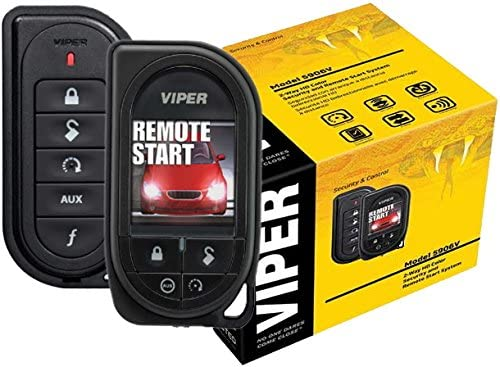
\includegraphics[width=0.8\textwidth]{images/viper_5906V_1.jpg}
			\caption{
				دستگاه
				\lr{remote control}
				به‌همراه جعبه.
			}
			\label{subfig1:fig1:sec3:chap1}
		\end{subfigure}
		\hspace*{1cm}
		\begin{subfigure}[t]{0.3\linewidth}
			\centering
			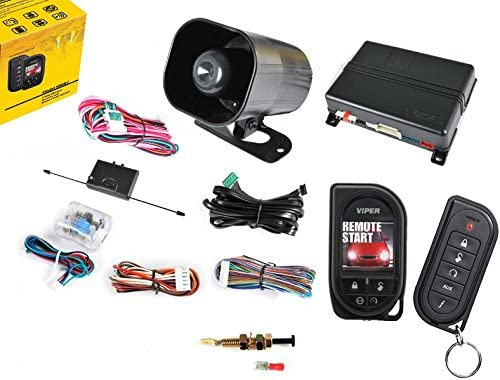
\includegraphics[width=0.8\textwidth]{images/viper_5906V_2.jpg}
			\caption{
				دستگاه 	به صورت
				\lr{unbox}
				شده، شامل ماژول‌ها
			}
			\label{subfig2:fig1:sec3:chap1}
		\end{subfigure}
		\\\vspace*{5mm}%% ----------------------------------------------------------------------
		\begin{subfigure}[t]{0.3\linewidth}
			\centering
			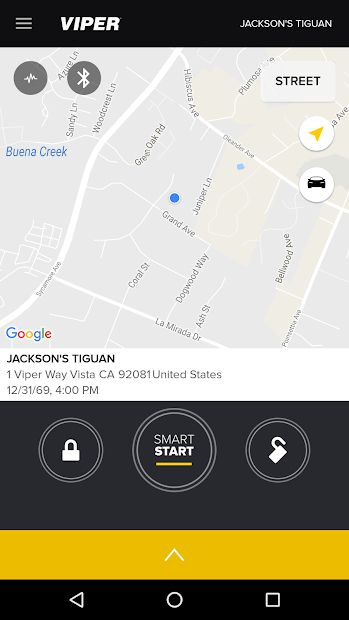
\includegraphics[width=0.8\textwidth]{images/viper_smart_start_1.jpg}
			\caption{
				صفحه نمایش موقعیت مکانی خودرو.
			}
			\label{subfig3:fig1:sec3:chap1}
		\end{subfigure}
		\hspace*{1cm}
		\begin{subfigure}[t]{0.3\linewidth}
			\centering
			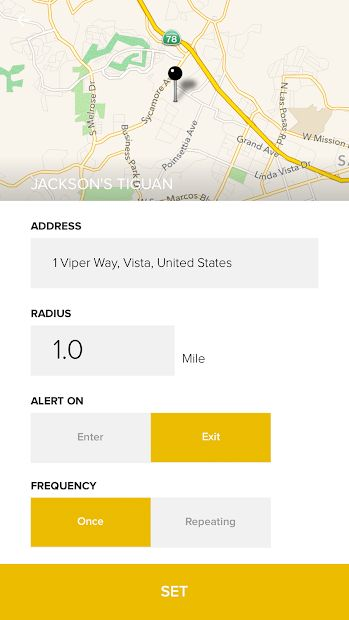
\includegraphics[width=0.8\textwidth]{images/viper_smart_start_2.jpg}
			\caption{
				صفحه مربوط به تنظیمات هشدار با توجه به موقعیت مکانی.
			}
			\label{subfig4:fig1:sec3:chap1}
		\end{subfigure}
		\normalsize
		\caption{
			عکس از جزئیات دزدگیر
			\lr{Viper 5906V}
			موجود در فروشگاه
			\hyperref{https://www.amazon.com/Viper-5906V-Color-Remote-Security/dp/B00H0874IG}{car alarm unboxed}{Viper 5906V}{\lr{amazon}}
		}
		\label{fig1:sec3:chap1}
	\end{figure}

	\lr{smart start}
	برنامه تلفن هوشمند ارائه شده توسط کمپانی
	\lr{viper}
	موجود در
	\hyperref{https://play.google.com/store/apps/details?id=com.directed.android.viper}{car alarm application}{Viper 5906V}{فروشگاه \lr{play}}
	که در
	\hyperref[fig1:sec3:chap1]{شکل 1.1}
	 در شکل‌های
	\hyperref[subfig3:fig1:sec3:chap1]{(ج)}
	و
	\hyperref[subfig3:fig1:sec3:chap1]{(د)}
	قابل مشاهده هستند.

	\subsubsection{
		امکانات
	}\label{subsubsec1:subsec1:sec3:chap1}
	\begin{itemize}[nosep]\label{item1:subsec1:sec3:chap1}
		\item
			محافظت از سرقت خودرو (مانند ایجاد هشدار و..).
		\item
			\lr{remote}
			 دوطرفه.
		\item
			رمزنگاری.
		\item
			روشن کردن خودرو به صورت
			\lr{remote}.
		\item
			داشتن نمایشگر
			\lr{OLED}
			در
			\lr{remote}.
		\item
			کنترل دمای داخلی خودرو.
		\item
			قفل درها به صورت اتوماتیک.
		\item
			برد
			\lr{remote}
				تا
			$1.5 km$
		\item
			ردیابی خودرو.
		\item
			استفاده از
			\lr{SST}\LTRfootnote{Spread Spectrum Technology.}
			برای ارتباط رادیویی.
		\item
			قابلیت اتصال به نرم‌افزار موبایل.
	\end{itemize}

	\subsection{
		\lr{Python 5760P}
	}\label{subsec2:sec3:chap1}

	دزدگیر
	\lr{Python 5760P}
	یکی دیگر از انواع
	\lr{remote}
	و  ساخته شده توسط کمپانی
	\lr{Directed Electronics}
	این دزدگیر هم مانند
	\lr{Viper 5906V}
	از امکانات مشابهی برخوردار است، که می‌توان مانند یک نسخه ارزان‌تر از محصول
	\lr{viper}
	دانست. این سیستم هشدار در سایت
	\lr{amazon}
		به قیمت
	$399.95\$$
	به فروش میرسد. از جمله دلایل قیمت پایین‌تر می‌توان به عدم وجود
	\lr{OLED}
	رنگی برای نمایش اطلاعات اشاره کرد.
	\cite{pythonHo3:online}

	\begin{figure}[!h]
		\begin{center}
			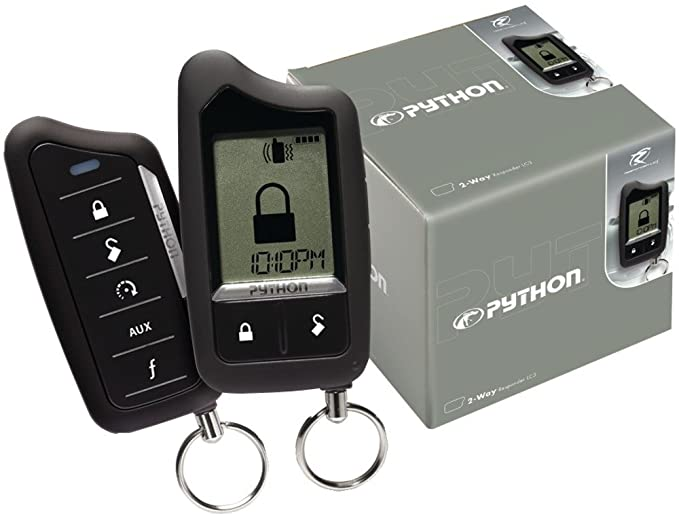
\includegraphics[width=0.4\textwidth]{images/Python_5760P.jpg}
			\caption{
			ریموت
			\lr{Python 5760P}}
			\label{fig1:subsec2:sec3:chap1}
		\end{center}
	\end{figure}
	\subsubsection{
		امکانات
	}\label{subsubsec1:subsec2:sec3:chap1}
	\begin{itemize}[nosep]\label{item1:subsec2:sec3:chap1}
		\item
		محافظت از سرقت خودرو (مانند ایجاد هشدار و..).
		\item
		رمزنگاری.
		\item
		قابلیت شخصی سازی حسگر‌ها.
		\item
		ردیابی خودرو.
		\item
		برد
		\lr{remote}
		تا
		$1.5 km$
		\item
		استفاده از
		\lr{SST}
		برای ارتباط رادیویی.
		\item
		قابلیت اتصال به نرم‌افزار موبایل، مشابه با
		\lr{Viper 5906V}
		از نرم‌افزار
		\lr{smart start}
		استفاده می‌کند که قبلاً معرفی شده.
	\end{itemize}

	\subsection{
		\lr{Avital 3100LX}
	}\label{subsec3:sec3:chap1}
	دستگاه
	\lr{carlock}
	یک دزدگیر و تحلیل‌گر خودرو است که به صورت یک
	\lr{gadget}
	به درگاه
	\lr{OBD}
	خودرو متصل می‌شود.
	این محصول به قیمت
	$49.95\$$
	فروشگاه
	\hyperref{https://www.amazon.com/gp/product/B00U0K3Q10}{car alarm}{carlock}{\lr{amazon}}
	به فروش می‌رسد.

	این دستگاه به صورت اینترنتی و پیامکی با تلفن ‌همراه ارتباط برقرار می‌کند که این خدمات باید به صورت جداگانه و سالانه با قیمت
	$120\$$
	خریداری شود، که یک ماه استفاده اولیه رایگان است.

	همچنین این محصول دارای
	\lr{tag}
	هایی برای باز شدن قفل خودرو در صورت ورود به محدوده خودرو است.

	که این
	\lr{tag}
	ها نیز به صورت جداگانه در فروشگاه
	\hyperref{https://www.amazon.com/CARLOCK-TAG-Accessory-ONLY-Automatically/dp/B075F4SWZ7}{car alarm}{carlocktag}{\lr{amazon}}
	به قیمت
	$19.90\$$
	به فروش می‌رسند.
	\cite{carAlarm:online}

	\hyperref[subfig2:fig2:subsec3:sec3:chap1]{شکل 	۱.۳}
	\begin{figure}[!h]
		\centering
		\footnotesize
		\begin{subfigure}[t]{0.3\linewidth}
			\centering
			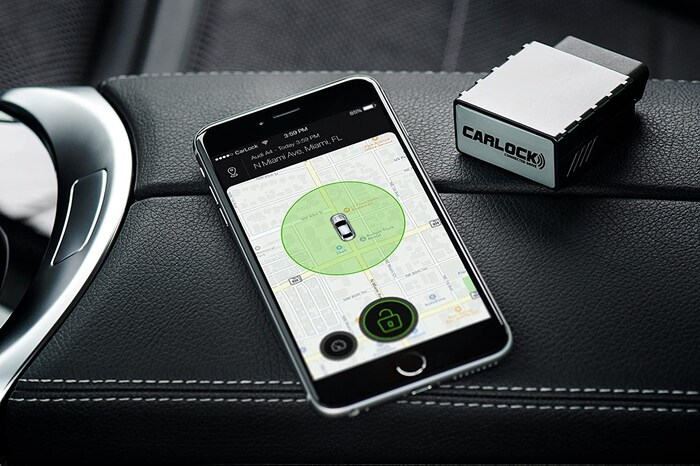
\includegraphics[width=0.8\textwidth]{images/carlock-main-module.jpeg}
			\caption{
				ماژول اصلی
				carlock.
			}
			\label{subfig1:fig1:subsec3:sec3:chap1}
		\end{subfigure}
		\hspace*{1cm}
		\begin{subfigure}[t]{0.3\linewidth}
			\centering
			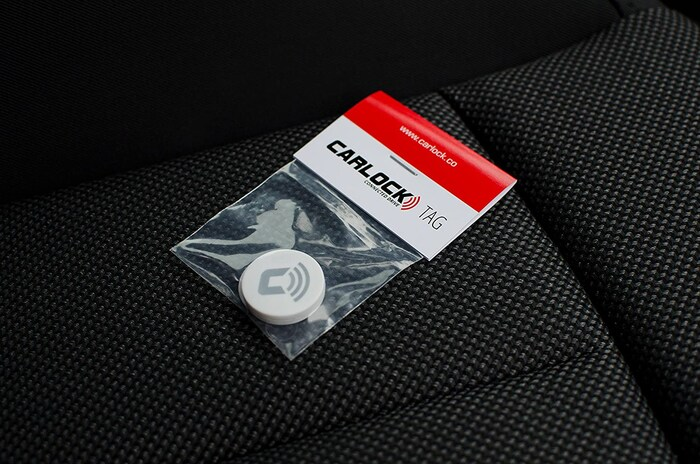
\includegraphics[width=0.8\textwidth]{images/carlock-tag.jpeg}
			\caption{
				\lr{carlock tag}
			برای باز شدن خودکار خودرو.
			}
			\label{subfig2:fig1:subsec3:sec3:chap1}
		\end{subfigure}\\
		\begin{subfigure}[t]{0.8\linewidth}
			\centering
			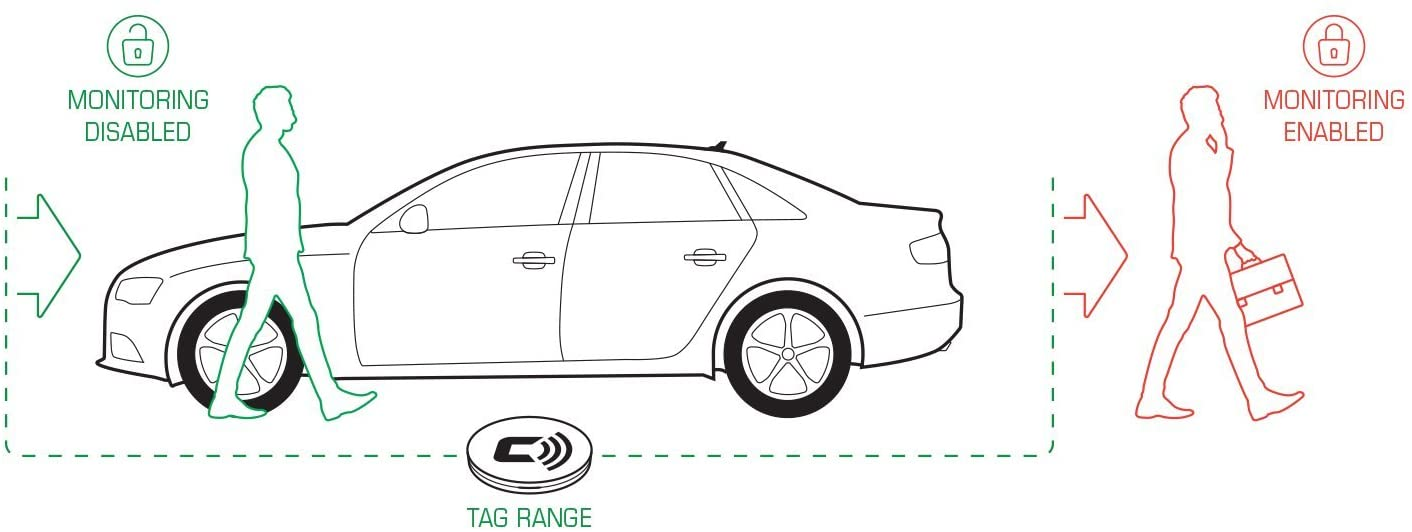
\includegraphics[width=0.93\textwidth]{images/carlock-tag-functionality.jpg}
			\caption{
				نحوهٔ عملکرد
				\lr{carlock tag}
				به صورت مصور.
			}
			\label{subfig1:fig2:subsec3:sec3:chap1}
		\end{subfigure}\\\vspace*{5mm}

		\begin{subfigure}[t]{0.8\linewidth}
			\centering
			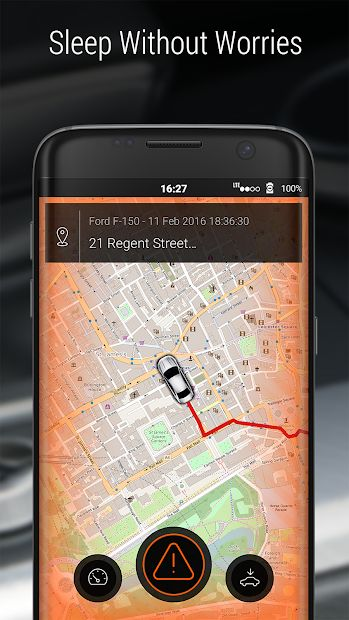
\includegraphics[width=0.3\textwidth]{images/carlock-app-ui-1.jpeg}
			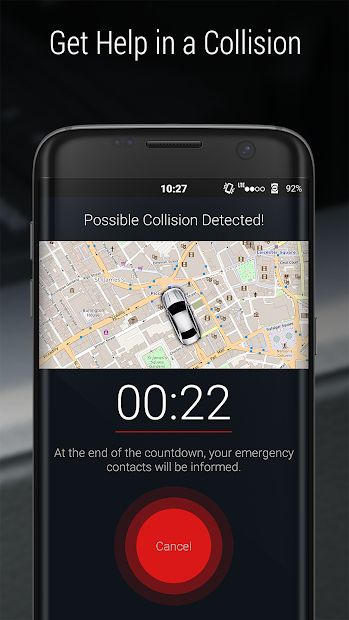
\includegraphics[width=0.3\textwidth]{images/carlock-app-ui-2.jpeg}
			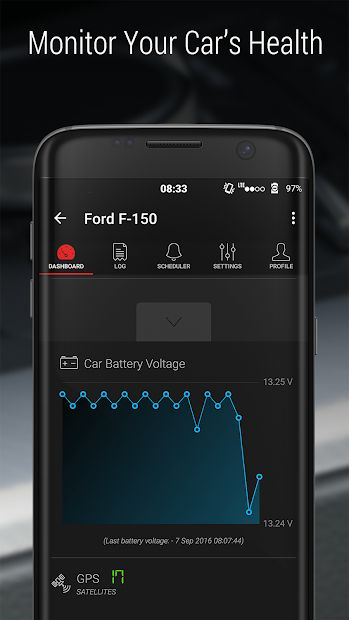
\includegraphics[width=0.3\textwidth]{images/carlock-app-ui-3.jpeg}
			\caption{
				نمایی از صفحات نرم‌افزار
				\lr{carlock}
				موجود در فروشگاه
				\lr{play}.
			}
			\label{subfig2:fig2:subsec3:sec3:chap1}
		\end{subfigure}
		\normalsize
		\caption{
			عکس‌ها و نمایه‌هایی
			\lr{application}
			مربوط به
			\lr{carlock}
			و ماژول‌های آن.
		}
		\label{fig2:subsec3:sec3:chap1}
	\end{figure}
	\subsubsection{
		امکانات
	}\label{subsubsec3:subsec3:sec3:chap1}
	\begin{itemize}[nosep]\label{item1:subsec3:sec2:chap1}
		\item
			ردیابی خودرو.
		\item
			گزارش وضعیت باتری.
		\item
			گزارش در صورت شوک و ضربه به خودرو.
		\item
			گزارش سرعت خودرو.
		\item
			قفل، و باز کردن در‌های خودرو.
		\item
			راه‌اندازی بسیار آسان با اتصال به پورت
			\lr{OBD}\LTRfootnote{On-board diagnostics}.
		\item
			گزارش لحظه‌ای از موقعیت خودرو در صورت سرقت.

	\end{itemize}

	\section{
	امکانات نهایی پروژه
	}\label{sec4:chap1}
	\begin{itemize}[nosep]\label{item1:sec4:chap1}
		\item
			ردیابی خودرو.
		\item
			کنترل برخی از عملکرد‌های خودرو.

			این بخش شامل عملکرد‌هایی که
			\lr{ECU}\LTRfootnote{engine control unit \TNR/endʒɪn kənˈtrəʊl ˈjuːnɪt/.}
			در اختیار قرار می‌دهد می‌باشد،‌ مانند جلوگیری از روشن شدن خودرو، یا خاموش کردن خودرو در صورت نیاز و تایید کاربر.
		\item
			گزارش وضعیت خودرو.
		\item
			کنترل ماژول اصلی به وسیله
			\lr{remote controller}.

			که شامل روشن‌کردن موقت خودرو، بازکردن درها و شیشه‌ها، هشدار اعلان خودرو و ... می‌باشد.
		\item
			اعمال پیشگیری از سرقت خودرو (مانند به صدا در آمدن هشدار و...)، که شامل امکانات ابتدایی در دزدگیر است.
		\item
			رمزنگاری ارتباط رادیویی و
			\lr{blutooth}.

			در این قسمت سعی می‌شود بهینه سازی‌هایی در ارسال دستورات
			\lr{remote}
			 از طریق ماژول رادیویی انجام داد.
	\end{itemize}
	\newpage
	\section{
		تکنولوژی‌های مورد استفاده
	}\label{sec5:chap1}

	\begin{enumerate}[nosep]\label{item1:sec5:chap1}
		\item
			\hyperref[subsec1:sec5:chap1]{\lr{Qt/C++}}
		\item
			\hyperref[subsec2:sec5:chap1]{\lr{QML}}
		\item
			\hyperref[subsec3:sec5:chap1]{\lr{ARM}}
	\end{enumerate}

	\subsection{\lr{Qt/C++}}\label{subsec1:sec5:chap1}
		فریم‌ورک
		\LTRfootnote{ freamwork\TNR /ˈfrāmˌwərk/.}
		محبوب
		\lr{Qt}\LTRfootnote{ Qt\TNR /kyo͞ot/.}
		که یکی از فریم‌ورک‌های زبان برنامه‌نویسی
		\lr{C++}
		است، و در این پروژه به منظور پیاده سازی
		\lr{android application}
		از آن استفاده می شود.

		فریم‌ورک
		\lr{Qt}
		به واسطه زبان قدرتمند
		\lr{C++}
		توانایی ایجاد
		\lr{source code}
		قابل حمل و چند سکویی

		را دارد.
		از طرفی این فریم‌ورک به خوبی می‌تواند با ترکیب
		\lr{QML}
		به عنوان زبان طراحی رابط کاربری و
		\lr{C++}
		برای سمت پردازش نرم‌افزار یک خروجی مناسب با رابط کاربری قابل پسند و کارایی مناسب ایجاد کند.
	\subsection{\lr{QML}}\label{subsec2:sec5:chap1}
	زبان
	\lr{QML}
	که از طرف شرکت
	\lr{Qt}
	به عنوان یک زبان مفسری با قابلیت استفاده از
	\lr{JS}\LTRfootnote{ Java Script\TNR\ /ˈjävəskript/.}،
	\lr{HTML}\LTRfootnote{ Hypertext Markup Language\TNR\ /ˈhīpərˌtekst ˈmärˌkəp ˈlaNGɡwij/.}
	و
	\lr{CSS}\LTRfootnote{ Cascading Style Sheet\TNR\ /kaˈskād stīl SHēt/.}
	در کد می‌توان به راحتی و با استفاده از این زبان یک رابط کاربری مناسب و زیبا ایجاد کرد.
	\cite{QtQML51548:online}
	\subsection{\lr{ARM}}\label{subsec3:sec5:chap1}
	\lr{ARM}\LTRfootnote{Acorn RISC Machine\TNR\ /ˈeɪˌkɔrn ˈrɪsk məˈʃiːn/ }
	یک پردازنده کامپیوتری از خانواده
	\lr{RISC}\LTRfootnote{Reduced Instruction Set Computing\TNR\ /rɪˈdjuːst ɪnˈstrʌkʃn̩ set kəmˈpjuːtɪŋ/.}
	است. که توسط کمپانی
	\lr{ARM}
	در حال توسعه است.
	این کمپانی اجازه ساخت و استفاده از این تکنولوژی را به کامپانی‌های دیگر نیز داده‌است،‌ محصولات خود از جمله سیستم‌های مبتنی بر چیپ‌ها
	(\lr{SoC}\LTRfootnote{System on Chips\TNR\ /ˈsɪstəm ˈɒn tʃɪps/.})
	و سیستم‌های مبتنی بر ماژول‌ها
	(\lr{SoM}\LTRfootnote{System on Modules\TNR\ /ˈsɪstəm ˈɒn ˈmɒdjuːlz/.})
	را پیاده سازی کنند. که از لحاظ مصرف انرژی، هزینه و اتلاف گرما کاملاً به صرفه است.

	همچنین این کمپانی هسته‌هایی را نیز طراحی می‌کند و اجازه آن را به شرکت‌هایی که نیاز به استفاده از
	هسته‌ها و  نسخه اصلی هسته
	(\lr{IP core\LTRfootnote{intellectual property core\TNR\ /ˌɪntəˈlektʃʊəl ˈprɒpəti kɔː/.}})
	 در محصولات خود را دارند می‌دهد.

	\subsubsection{
		میکروکنترلر
		\lr{STM32F103}}
	میکروکنترلر
	\lr{STM32F103}
	از خانواده تراکم متوسط با عملکرد خطی، شامل پردازنده
	\lr{ARM}
	با عملکرد بالا از نوع هسته 32 بیت و از قشر
	\lr{M3}
	با فرکانس تا
	$ 72 MHz $
	و حافظه فوق سریع تا
	$ 128 Kbytes $
	دارای
	$ 48 pin $
	شامل دو
	\lr{ADC}
	$ 12-bit $
	، سه تایمر
	$ 16-bit $
	و یک
	\lr{PWM}
	و شامل دو
	\lr{I2C}
	و
	\lr{SPI}
	با ولتاژ کاری 2 تا $ 3.7 $ ولت است.
	\cite{ltc3600:datasheet}

	دیگر ماژول‌های مورد استفاده در این پروژه شامل:
	\begin{itemize}[nosep]\label{item2:sec5:chap1}
		\item
		یک ماژول
		\lr{SIM800L}
		برای اتصال به شبکه موبایل.
		\item
		و ماژول
		\lr{GYNEO6MV2}
		برای موقعیت یابی به وسیله
		\lr{GPS}.
		\item
		به همراه چند ماژول ارتباط رادیویی و
		\lr{blutooth}
		برای ارتباط و کنترل از طریق دستگاه
		\lr{remote}
		و تلفن همراه.
	\end{itemize}

	از دلایل انتخاب میکروکنترلر
	\lr{ARM}
	قیمت پایین و مصرف انرژی بسیار پایین و همچنین داشتن واحد‌های پردازشی بیشتر نسبت به
	\lr{AVR}
	و دیگر میکروکنترلرها است.

	برای طراحی مدار نیز نرم‌افزار
	\lr{Altium Designer}
	مد نظر قرار گرفته شده‌است که محیط مناسب برای طراحی حرفه‌ای مدار را فراهم می‌کند.
	\pagebreak
	\opchapter{
    تحلیل پروژه
}\label{chap2}

\section{
    مقدمه
}\label{sec1:chap2}


\section{
    متدولوژی کنبان
}\label{sec2:chap2}
\lr{kanban}
\footnote{کَنبان.}
یک روش مدیریت چرخهٔ کار برای تعریف، مدیریت و بهبود سرویس‌های انتقال دانش کار است.
که هدف آن کمک برای متصور سازی، افزایش بهره‌وری و بهبود متداوم کار می‌باشد.

کنبان در زبان ژاپنی به معنی
\emph{تختهٔ بصری}
و یا
\emph{علامت}
است.
در ابتدا به عنوان یک سیستم برنامه‌ریزی به عنوان مدیریت ناب
\LTRfootnote{lean manufacturing \TNR\ /ˈli:n ˌmænjʊˈfæktʃərɪŋ/}
در سال
$1940$
توسط
\lr{Toyota}\footnote{
    تویوتا، یک ‌شرکت خودروسازی ژاپنی تأسیس شده در سال
    $1935$.
}
مطرح شد، که از سیستم همزمان
\lr{Toyota}
الهام گرفته شد، که بعد‌ها در سال
$2007$
به عنوان روش کنبان پدید آمد.
\cite{ohno1988toyota:book}
در متدولوژی کنبان از یک تخته کنبان استفاده می‌شود. 	در حالت ساده این تخته شامل $3$ ستون انجام دادن
(\lr{To-Do})،
در حال انجام
(\lr{In Progress})
و انجام شده
(\lr{Done})
است، که ممکن است شامل ستون‌های بانک اطلاعاتی
(\lr{Backlog})،
آماده انجام
(\lr{Ready})،
کد زنی
(\lr{Coding})،
آزمایش
(\lr{Testing})،
و تأ‌یید
(\lr{Approval})
نیز باشد.
\cite{kanbanize:online}

\emph{
کنبان برای یک
}\LTRfootnote{Kanban For 1.}،
یک روش الهام گرفته شده از کنبان مناسب برای توسعهٔ پروژه‌هایی با یک توسعه‌دهنده است.
\cite{prsonalkanban:online}
\begin{figure}[!h]
    \begin{center}
        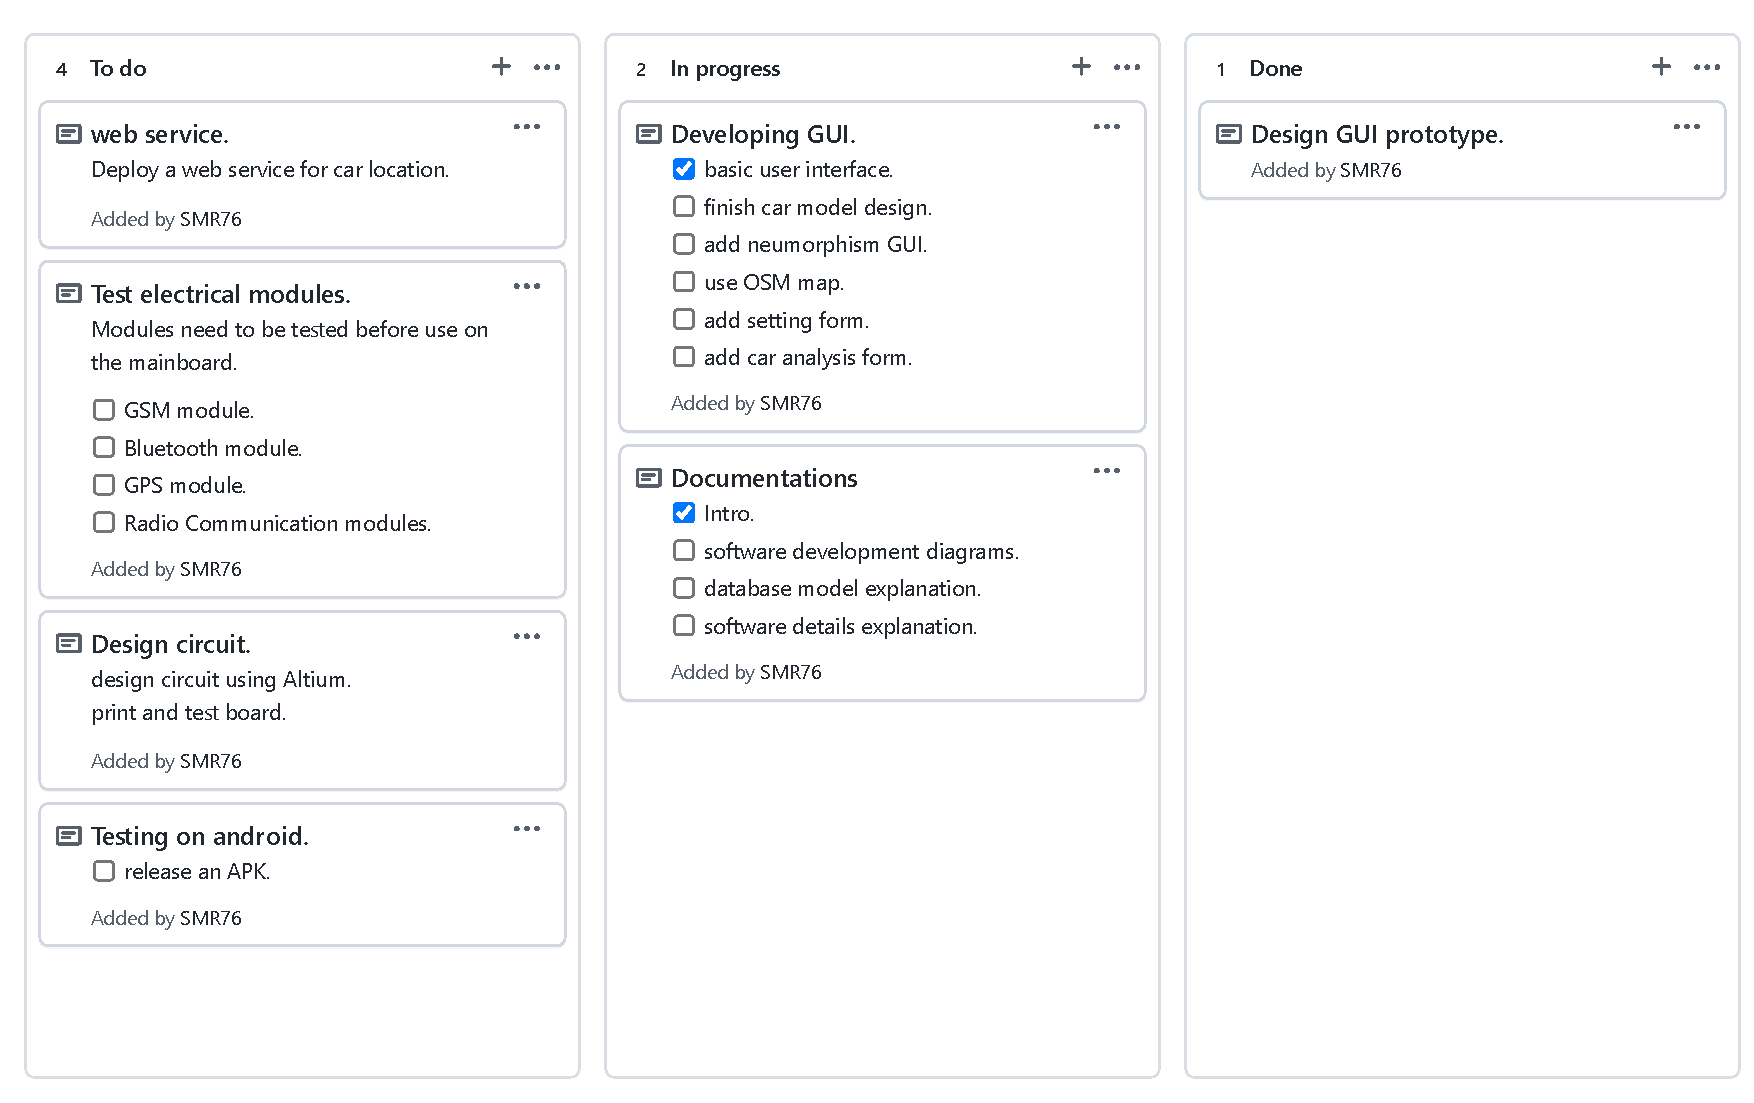
\includegraphics[width=0.8\textwidth]{images/kanban-board.pdf}
    \end{center}
    \caption{
        نمونهٔ تختهٔ کنبان در پروژهٔ جاری.
    }
    \label{fig3:sec1:chap2}
\end{figure}

\section{
    نمودار فعالیت
}\label{sec4:chap2}
نمودار فعالیت شامل عملکرد کاربر و طریقه انجام مراحل و گزینه‌های موجود پیش روی است.
این نمودار خلاصه‌ای از عملیات‌های موجود و قابل انجام توسط دستگاه را توضیح می‌دهد.

\begin{figure}[!h]
    \begin{center}
        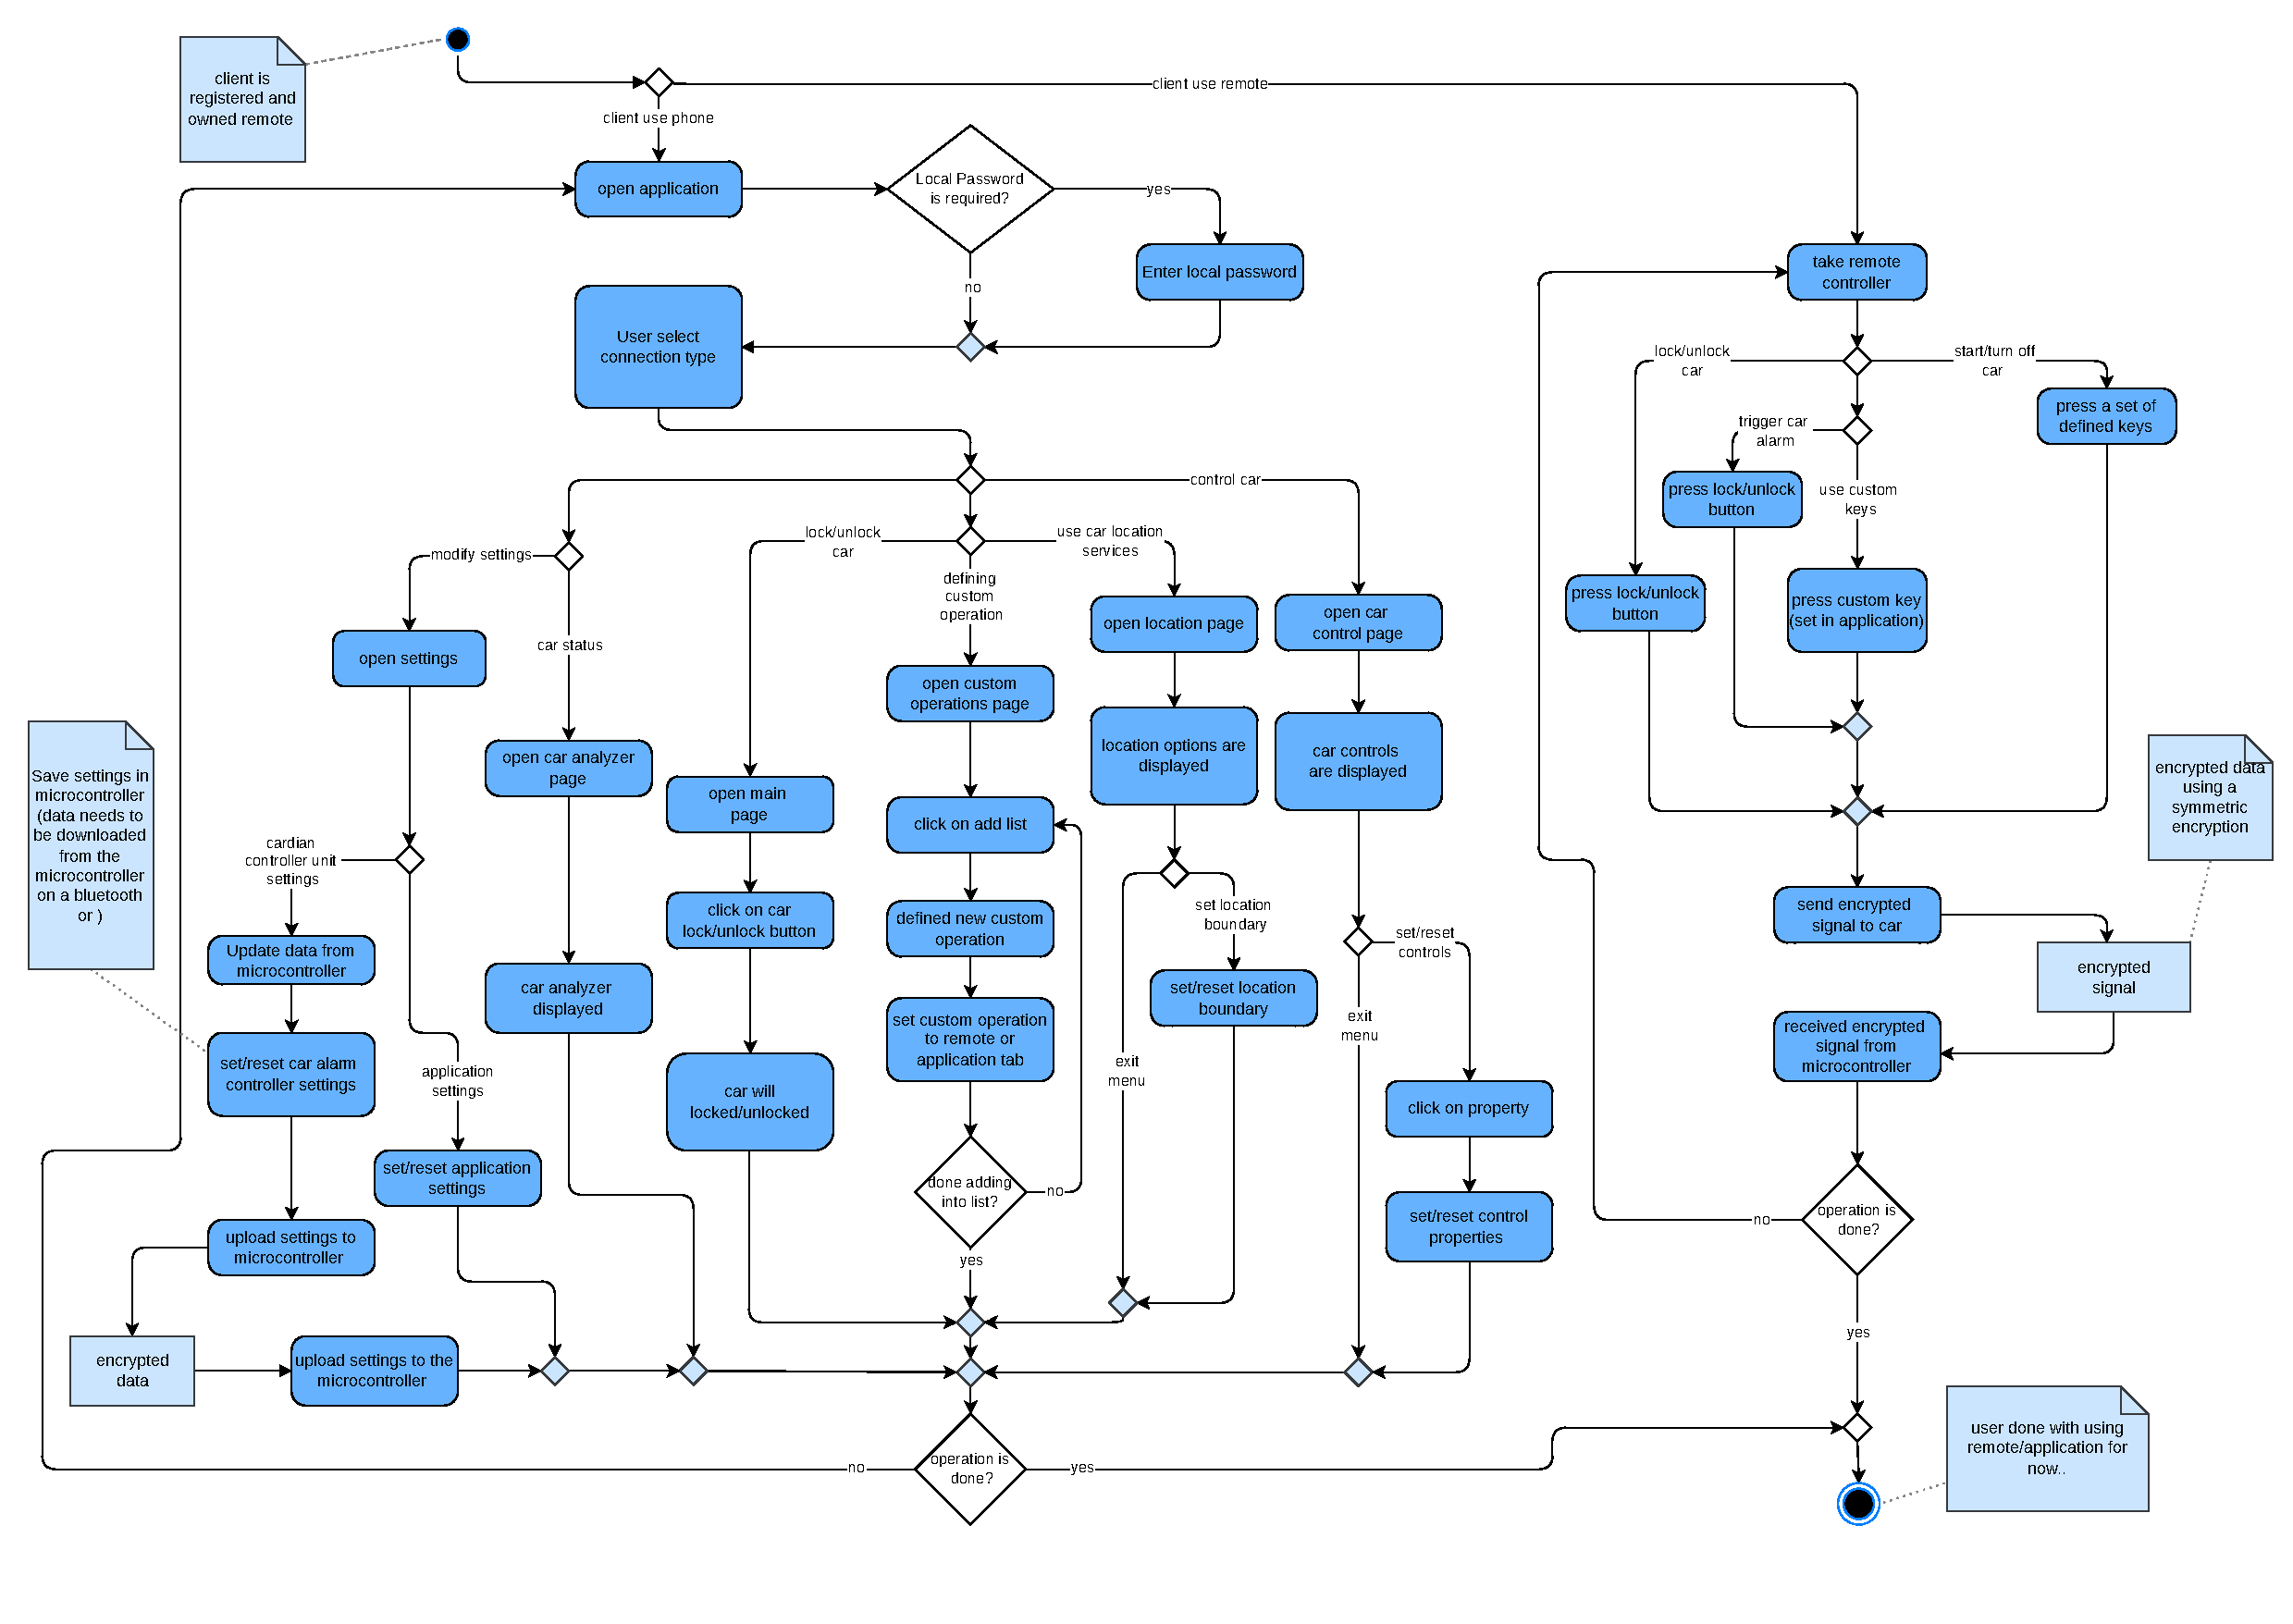
\includegraphics[width=0.8\textwidth]{../diagrams/activity-diagram.pdf}
        %../Extera/SD Diagrams/UML/activity-diagram.pdf
    \end{center}
    \caption{
    نمودار فعالیت.
    }
    \label{fig4:sec1:chap1}
\end{figure}

\pagebreak
\section{
    نمودار مدل و نشانه‌گذاری فرایند کسب‌وکار
}\label{sec5:chap2}

نمودار مدل و نشانه‌گذاری فرایند کسب‌وکار
(\lr{BPMN}\LTRfootnote{Business Process Model and Notation})
 یک نمودار گرافیکی است که برای نمایش و توصیف فرایندهای کسب و کار در یک سازمان استفاده می‌شود. این نمودارها با استفاده از یک مجموعه عناصر گرافیکی و قوانین نمونه سازی، نحوه جریان اطلاعات و وظایف در یک فرایند را نمایش می‌دهند.

نمودار
\lr{BPMN}
ترکیبی از اشکال گرافیکی و نمادهای استاندارد است که برای نشان دادن وظایف، دروازه‌ها، رویدادها، شروع و پایان فرایند، و نقش‌های مختلف در فرایند استفاده می‌شوند.

در زیر نمودار‌های از چند فرایند پروژه نمایش داده شده‌است:

\begin{figure}[!ht]
    \centering
    \footnotesize
    \begin{subfigure}[t]{0.47\linewidth}
        \centering
        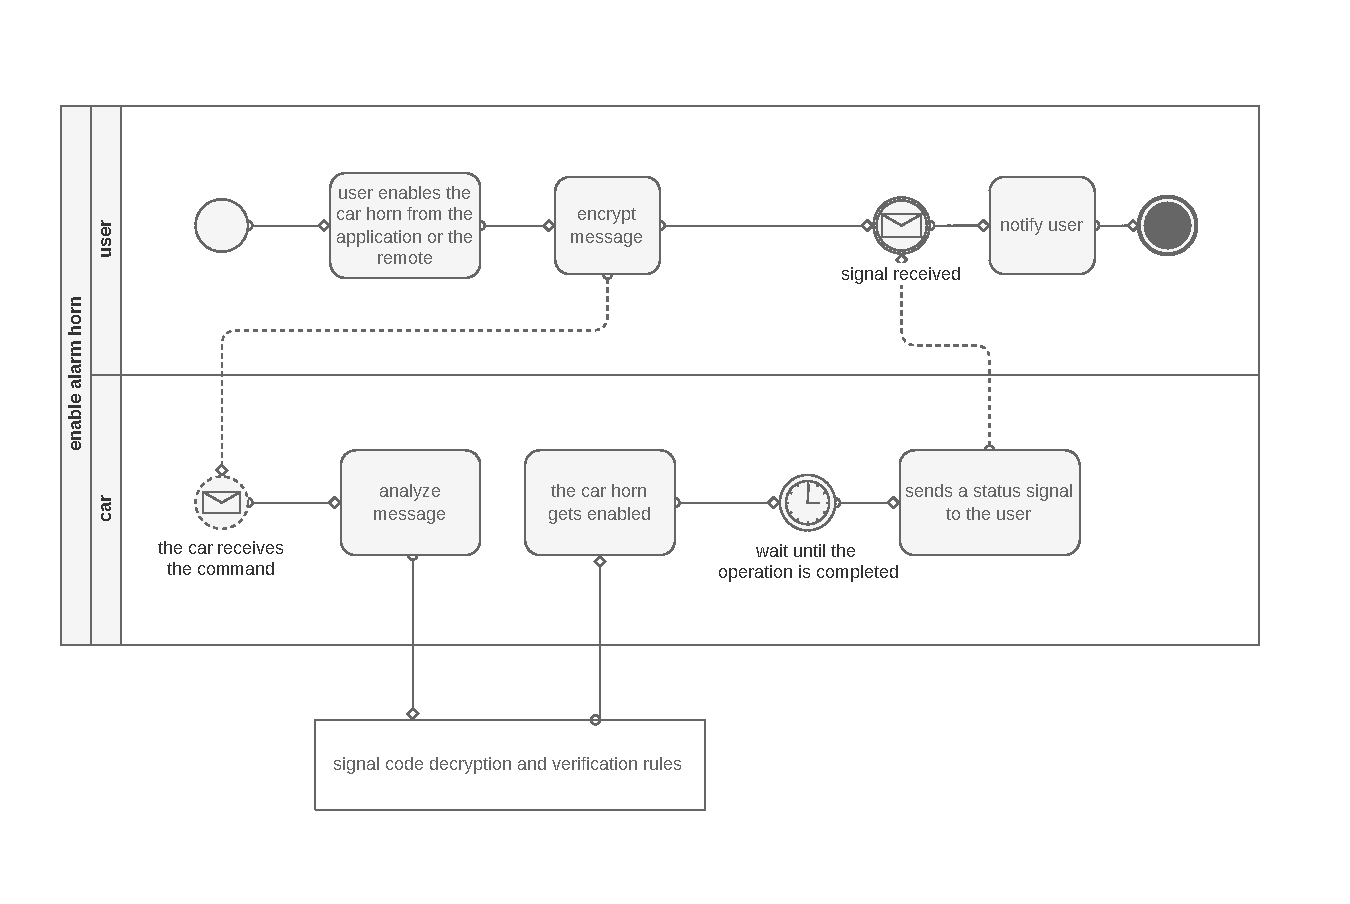
\includegraphics[width=\textwidth]{../diagrams/bpmn-diagram-1.pdf}
        \caption{
        فعال‌سازی آژیر خودرو
        }
        \label{subfig1:fig5:sec5:chap2}
    \end{subfigure}
    \begin{subfigure}[t]{0.47\linewidth}
        \centering
        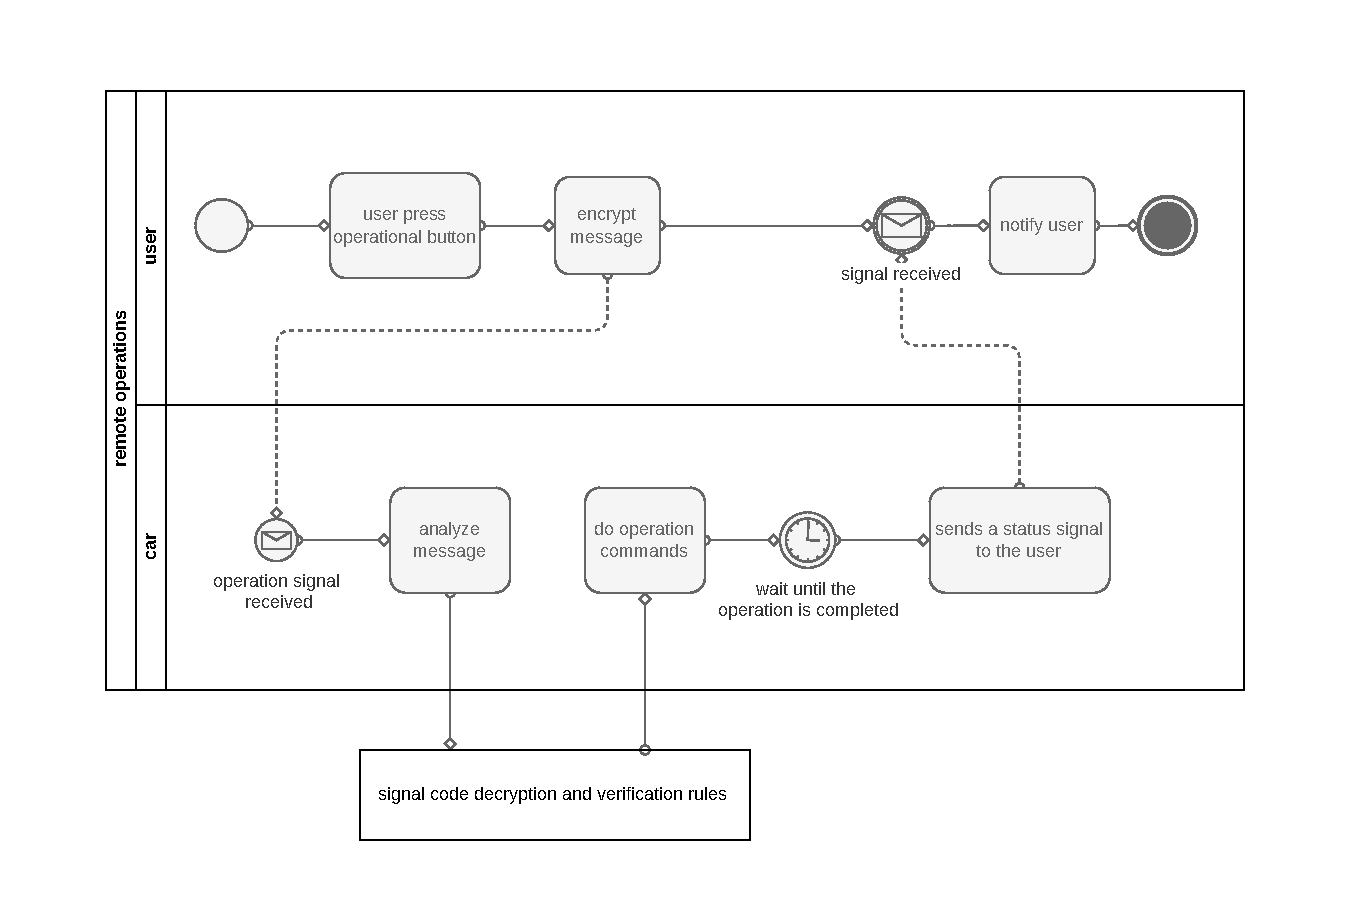
\includegraphics[width=\textwidth]{../diagrams/bpmn-diagram-2.pdf}
        \caption{
            مراحل کنترل از راه‌دور  خودرو
        }
        \label{subfig2:fig5:sec5:chap2}
    \end{subfigure}
    \hspace*{1cm}
    \normalsize
    \label{fig5:sec5:chap2}
    \caption{
        نمودار
        \lr{BPMN}
        بخش
        $2$
    }
\end{figure}

\begin{figure}[!ht]
    \centering
    \footnotesize
    \begin{subfigure}[t]{0.47\linewidth}
        \centering
        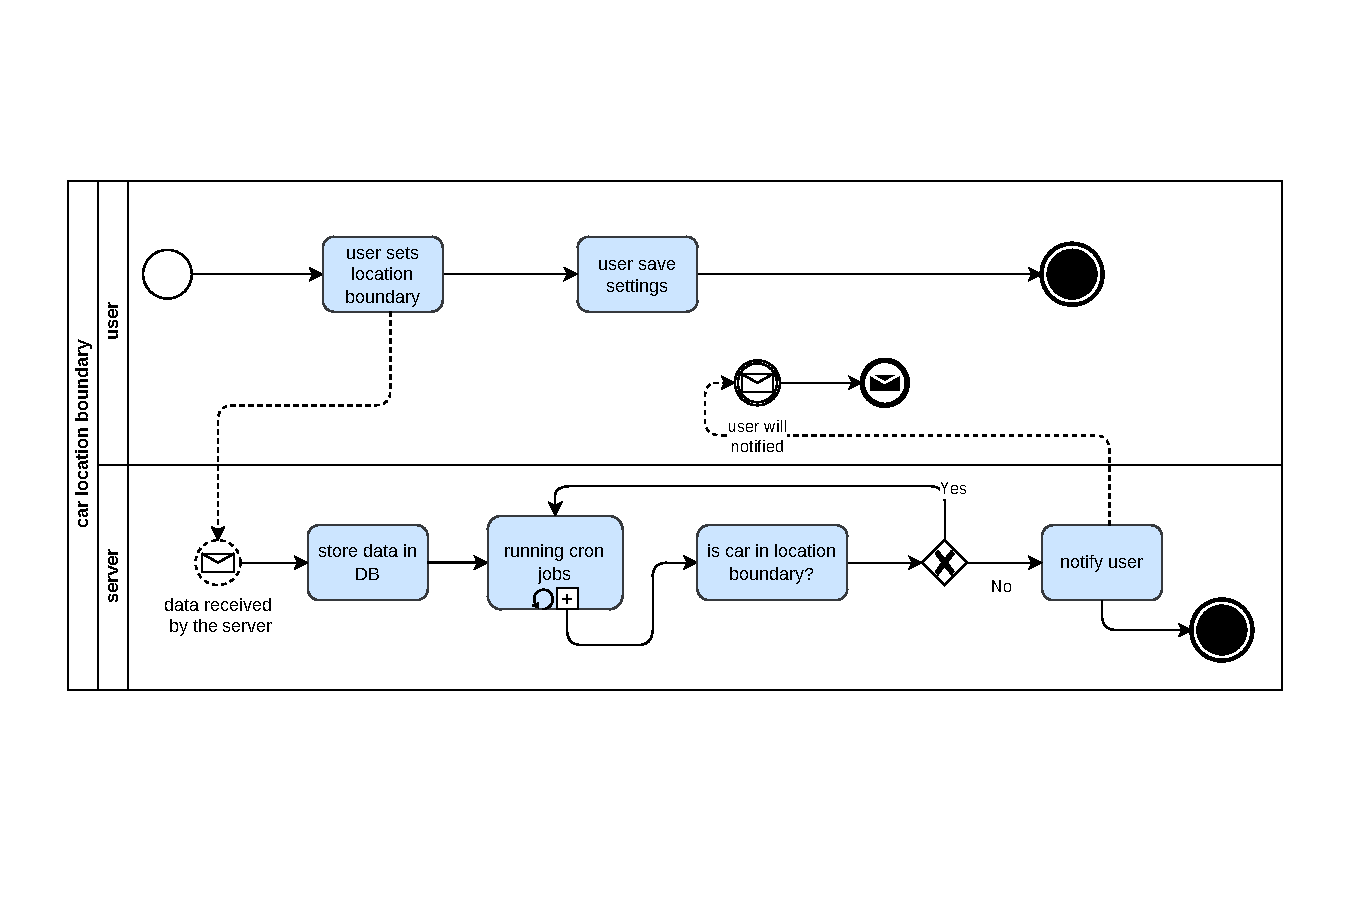
\includegraphics[width=\textwidth]{../diagrams/bpmn-diagram-3.pdf}
        \caption{
            قرار دادن محدودیت منطقه‌ای برای خودرو
        }
        \label{subfig1:fig6:sec5:chap2}
    \end{subfigure}
    \begin{subfigure}[t]{0.47\linewidth}
        \centering
        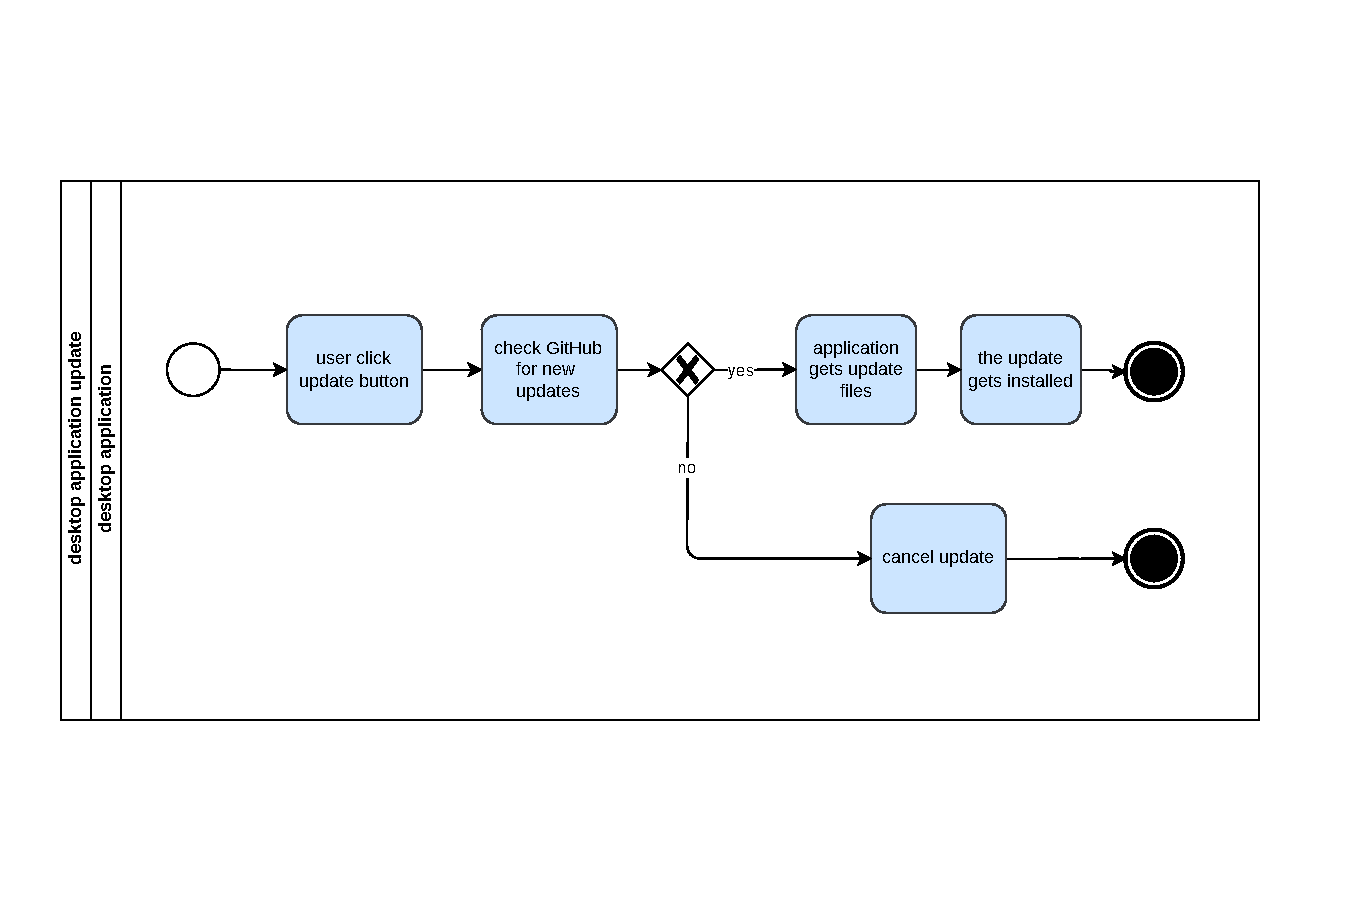
\includegraphics[width=\textwidth]{../diagrams/bpmn-diagram-4.pdf}
        \caption{
            به‌روزرسانی برنامهٔ
            \lr{desktop}
        }
        \label{subfig2:fig6:sec5:chap2}
    \end{subfigure}
    \hspace*{1cm}
    \normalsize
    \label{fig6:sec5:chap2}
    \caption{
        نمودار
        \lr{BPMN}
        بخش
        $1$
    }
\end{figure}

	\pagebreak
	
\opchapter{پایگاه داده}\label{chap3}

\section{تعریف}\label{sec1:chap3}

پایگاه دادهٔ
\lr{MySQL}\footnote{MySQL:‌ \TNR/mai.es·kyoo·el/}
 یک سیستم مدیریت پایگاه داده رابطه‌ای (\lr{RDBMS}) است که برای ذخیره، مدیریت و دسترسی به داده‌ها استفاده می‌شود. \lr{MySQL} یکی از پایگاه‌های داده محبوب و قدرتمند است که توسط شرکت \lr{Oracle} توسعه داده شده است. این پایگاه داده از زبان ساختار یافته پرس و جو (\lr{SQL}) برای تعامل با داده‌ها استفاده می‌کند.

\lr{MySQL} امکانات گوناگونی را برای مدیریت پایگاه داده فراهم می‌کند، از جمله:

\begin{itemize}[nosep]
	\def\labelenumi{\arabic{enumi}.}

	\item
	ایجاد و مدیریت جداول.
	\item
	جستجو و استخراج داده‌ها.
	\item
	نظارت بر امنیت.
	\item
	پشتیبانی از تراکنش‌ها.
	\item
	پشتیبانی از اتصال همزمان.
	\item
	پشتیبانی از رویکردهای بالا.
\end{itemize}

با این تعریف پایگاه دادهٔ \lr{MySQL} را می‌توان یک سیستم مدیریت پایگاه داده
رابطه‌ای محبوب و قدرتمند دسته بندی کرد که از زبان \lr{SQL} برای مدیریت داده‌ها
استفاده می‌کند و امکانات زیادی را برای طراحی، مدیریت و استفاده از پایگاه
داده‌ها فراهم می‌کند.

در اینجا از \lr{MySQL} در سمت \lr{server} استفاده شده و اطلاعات کاربران، توکن‌های
دسترسی، فراداده‌های کاربران، دستورات ارسال شده توسط دستگاه‌های سمت کاربر و
همچنین لیست وضعیت‌های رخ داده و در حال رخ دادن در خودرو ذخیره شده‌اند.


\paragraph{توابع تحلیل فضایی}\label{par1:sec1:chap3}

\lr{MySQL} دارای قابلیت ذخیرهٔ \lr{polygon}های جغرافیایی است که اجازه می‌دهد تا
نقاط و شکل‌های هندسی چندضلعی را در جداول دیتابیس ذخیره کند و عملیات
محاسبات مکانی را روی آن‌ها انجام دهد.

اضافه بر موارد گفته شده، یکی از قابلیت‌های مفید \lr{MySQL} وجود توابع تحلیل
فضایی
\LTRfootnote{Spatial Analysis Functions.}
 است. که امکان ذخیره‌سازی محدوده‌های
جغرافیایی مشخص‌شده توسط کاربر محیا می‌کند، و همچنین امکان اجرای یک \lr{query}
برای بررسی وجود یک نقطه درون آن محدوده، که در اینجا برای تشخیص وجود
خودرو در محدودهٔ مشخص شده توسط کاربر استفاده شده‌است.

در مجموع ویژگی‌های موجود عبارت‌اند از:

\begin{itemize}[nosep]
	\item
	نوع داده: در \lr{MySQL}، \lr{polygon}های جغرافیایی به صورت اشیاء جغرافیایی ذخیره
	می‌شوند. این شئ می‌تواند یک چندضلعی بسته، یک لایه منطقی یا یک نقشه در
	نظر گرفته شود.
	\item
	ذخیرهٔ داده: پلتفرم \lr{GIS} از جداول داده‌های جغرافیایی به عنوان کشویی برای
	ذخیرهٔ اشیاء جغرافیایی استفاده می‌کند. به همین دلیل، می‌توانید
	\lr{polygon}های جغرافیایی را به صورت \lr{filed} در جداول خود ذخیره کنید.
	\item
	عملیات مکانی: یکی از ویژگی‌های قوی \lr{MySQL} امکان انجام عملیات مکانی روی
	داده‌های جغرافیایی است. با استفاده از توابع مکانی مانند \lr{ST\_Contains}،
	\lr{ST\_Intersects} و \lr{ST\_Distance}، می‌توانید عملیات پرس‌وجوی پیچیده را روی
	\lr{polygon}هایی که در جداول ذخیره شده‌اند، انجام دهید.
	\item
	هندسه مکانی:
	\lr{MySQL}
	 قادر به ارائهٔ ویژگی‌های هندسی مانند محاسبهٔ مساحت و
	محدودهٔ \lr{polygon}های جغرافیایی است. توابعی مانند \lr{ST\_Area}، \lr{ST\_Length} و
	\lr{ST\_Perimeter} این امکان را فراهم می‌کنند.
\end{itemize}

بنابراین، به کمک قابلیت ذخیرهٔ \lr{polygon}های جغرافیایی در \lr{MySQL} می‌توانید
منطق مکانی و پرس‌وجوی پیچیدهٔ وابسته به مکان را در سیستم‌های خود پیاده‌سازی
کنید.


\subsection{جداول پایگاه‌داده}\label{sub1:sec1:chap3}

لیست جداول تعریف شده در سمت \lr{server} به صورت ذیل است.

از طرفی به دلیل افزایش کارایی اجرا و سرعت بیشتر و همچنین سبکی سعی شده
جداول حدالامکان ساده طراحی و مشخص شده‌باشند و اطلاعات به راحتی قابل
پرس‌وجو توسط \lr{MySQL} باشند.

همچنین برای ذخیرهٔ نشست‌های کاربران از برنامه‌های موجود همانند
\lr{Telegram}\footnote{
	تلگرام یک برنامهٔ شبکهٔ اجتماعی و یک پیام‌رسان است.
}
ایده گرفته شده و قابلیت تمایز و اتصال چند نشست از طرف یک کاربر ممکن است،
و همچنین اطلاعات کاربران مشابه به ذخیرهٔ اطلاعات به صورت عمومی‌تر و امکان
تغییر راحت‌تر به صورت یک جدول از کلید و داده
(\lr{key/value}) ذخیره شده‌اند،‌این
عمل از ذخیرهٔ‌ داده‌ها در
\lr{WordPress}\footnote{
	وردپرس یک
	\lr{CMS}
	محبوب برای ساخت وبسایت‌ها است.
}
ایده‌برداری شده.

\subsection{لیست جداول و توضیحات مربوط}\label{sub2:sec1:chap3}

\begin{itemize}[nosep]
	\item
	نوع دستگاه (\lr{device\_type}) در این جدول نوع دستگاه‌های ممکن لیست شده،‌که
	به صورت پیش‌فرض شامل \lr{vehicle}، \lr{android}، \lr{linux}، \lr{win}، \lr{ios} است.

	\textbf{ویژگی‌ها}: شناسه (\lr{id}), نام (\lr{name}), توضیحات (\lr{desc})
	\item
	حالت (\lr{states})

	حالت‌های موجود برای هر دستور، محدوده یا کاربر، که به صورت پیش‌فرض شامل
	مقادیر \lr{activated}، \lr{disabled}، \lr{suspended}، \lr{readonly} است.

	\textbf{ویژگی‌ها}: شناسه (\lr{id}), نام (\lr{name}), توضیحات (\lr{desc})
	\item
	نوع وضعیت و دستورات (\lr{fields})

	این جدول شامل نوع وضعیت‌ها و دستورات موجود در جدول‌های \lr{statuses} و
	\lr{commands} است.

	داده‌های در این دو جدول به صورت \lr{JSON} برای راحتی تلفیق و همچنین راحتی
	تعریف انواع دادهٔ جدید در صورت نیاز تعریف شده، که به واسطهٔ این جدول
	امکان دسته‌بندی راحت‌تر داده‌ها در جدول \lr{commands} را ممکن می‌سازد.

	\textbf{ویژگی‌ها}: شناسه (\lr{id}), نام (\lr{name}), توضیحات (\lr{desc})
	\item
	کاربران (\lr{users})

	جدول کاربران شامل شناسهٔ کاربر، توکن (\lr{token}) دسترسی و همچنین آخرین
	زمان دسترسی کاربر است.

	\textbf{ویژگی‌ها}: شناسه (\lr{id}), وضعیت (\lr{stid}), توکن (\lr{token}), زمان (\lr{utc})
	\item
	نشست‌های کاربران (\lr{users\_sessions})

	برای ایجاد دستورات و ارسال داده به سرور هر کاربر با توجه به هر دستگاه
	نیازمند ایجاد یک نشست برای دستگاه موجود است، بدین حالت بعد از ایجاد
	نشست کاربر از توکن احراز هویت خود برای ورود به سیستم استفاده کند.

	همچنین در این جدول برخی از ویژگی‌های مهم‌تر دستگاه مقصد نیز نگه‌داری
	می‌شوند.

	\textbf{ویژگی‌ها}: شناسه (\lr{id}), کاربر (\lr{uid}), نوع دستگاه(\lr{tid}), وضعیت
	(\lr{stid}), توکن احراز هویت (\lr{authtoken}), شناسهٔ یکتای دستگاه (\lr{mac}), زمان
	ایجاد (\lr{register}), زمان آخرین دسترسی (\lr{access}), آدرس \lr{IP} دستگاه (\lr{ip}),
	(\lr{port})
	\item
	محدوده‌های مشخص شده(\lr{boundaries})

	محدوده‌های مشخص شده به کاربر اجازهٔ ایجاد بخش‌ها و محدوده‌های جغرافیایی   را می‌دهد، که توانایی ایجاد رفتارهای متفاوت را به کاربر برای هر بخش را   بدهند.

	\textbf{ویژگی‌ها}: شناسه (\lr{id}), جلسه (\lr{sid}), وضعیت (\lr{stid}), محدودهٔ
	جغرافیایی (\lr{poly}), زمان (\lr{utc})
	\item
	آخرین وضعیت خودرو (\lr{latest\_status})

	آخرین وضعیت خودرو شامل یک مقدار \lr{JSON} است که شامل داده‌های تجمیع شده از آخرین وضعیت خودرو است، که برای دسترسی سریع‌تر و نیاز به بررسی تمامی  دستورات موجود را مهیا می‌کند.

	\textbf{ویژگی‌ها}: شناسه (\lr{id}), کاربر (\lr{uid}), مجموعهٔ آخرین تغییرات در یک
	جا به صورت \lr{JSON} (\lr{data}), زمان (\lr{utc})
	\item
	تمام وضعیت‌های گزارش شده (\lr{statuses})

	در این جدول وضعیت‌های گزارش‌ها توسط هر خودرو لیست شده‌اند.

	\textbf{ویژگی‌ها}: شناسه (\lr{id}), جلسه (\lr{sid}), نوع مقدار (\lr{fid}), محتوا به
	صورت \lr{JSON} (\lr{data}), زمان (\lr{utc}), وضعیت دسترسی و مشاهده (\lr{accessed})
	\item
	دستورات ارسال شده (\lr{commands})

	این جدول شامل دستورات ارسال شده توسط کاربر است، دستورات ارسال شده در   قالب \lr{JSON} هستند، برای مثال: نمونه‌ای از دادهٔ یک دستور برابر
	‍‍\lrm{\{"doors":{[}false,false,false,false{]}\}} است.

	\textbf{ویژگی‌ها}: شناسه (\lr{id}), جلسه (\lr{sid}), نوع مقدار (\lr{fid}), محتوا به
	صورت \lr{JSON} (\lr{data}), زمان (\lr{utc}), وضعیت دسترسی و مشاهده (\lr{accessed})
	\item
	فرادهده‌های مربوط به هر کاربر (\lrm{user\_meta})

	مشابه به هر سیستمی هر کاربر شامل فرا‌داده‌هایی مانند پست الکترونیکی، شمارهٔ همراه و
	\ldots{}
	 است که این جدول برای ذخیرهٔ این نوع از داده‌ها   قرار گرفته، که داده‌ها به صورت ترکیبی از کلید و داده در این جدول ذخیره   شده‌اند، که یک رابطهٔ یک به چند با جدول کاربر دارد.

	\textbf{ویژگی‌ها}:
	شناسه (\lr{id}), کاربر (\lr{uid}), نام فرا داده (\lr{key}), مقدار   فرا داده (\lr{value})
\end{itemize}

\section{دیاگرام}\label{sec2:chap3}
در ذیل دیاگرام مربوط به جداول پایگاه‌دادهٔ ایجاد شده در سمت سرور فراهم شده‌است.
که شامل ۸ جدول مرتبط به هم هستند.
\begin{figure}[!h]
	\centering
	\footnotesize
	\frame{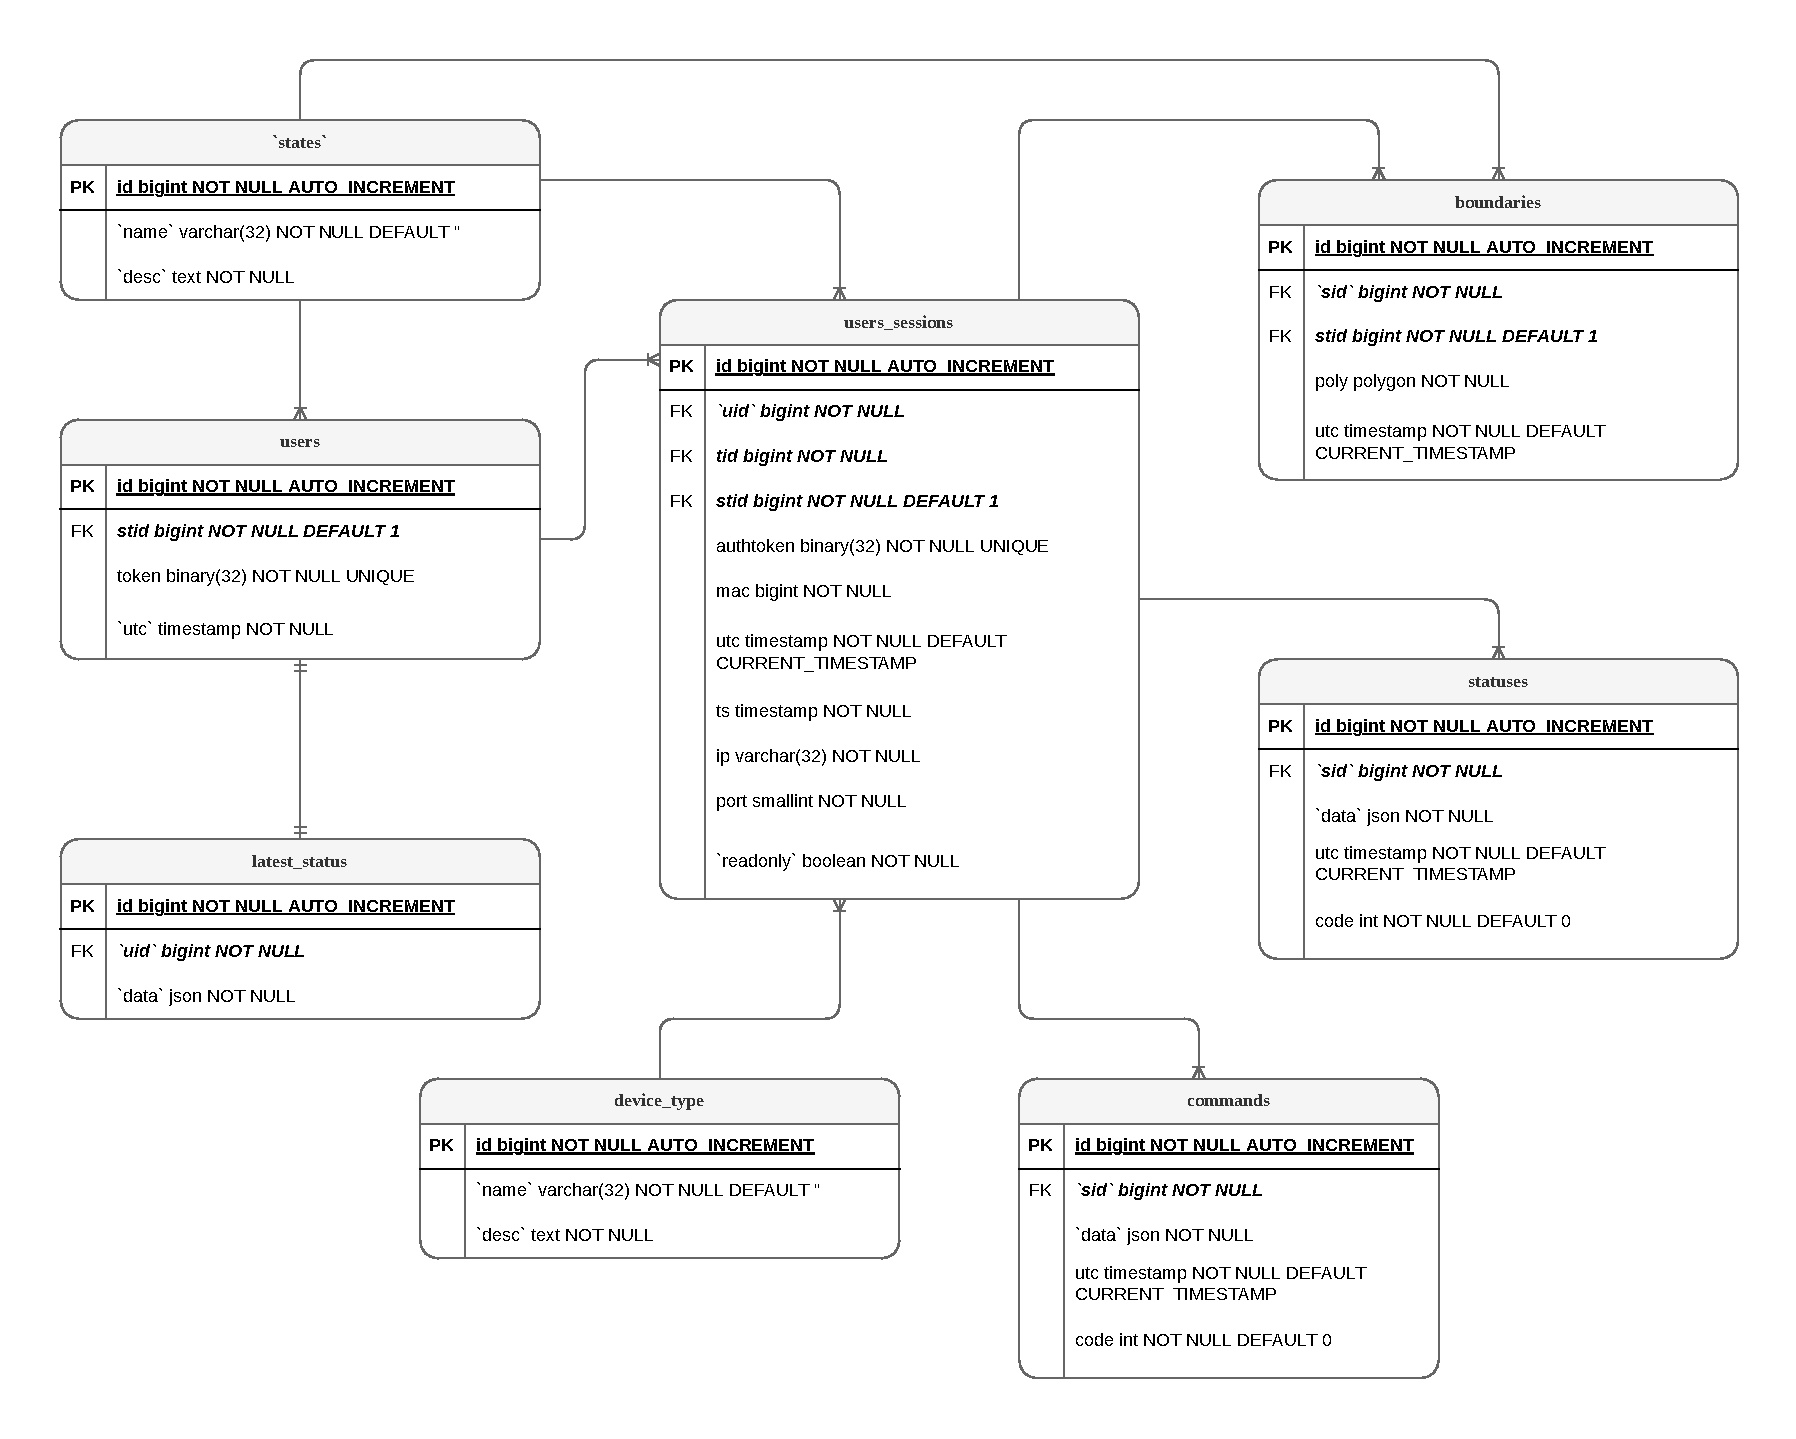
\includegraphics[width=\textwidth]{../diagrams/database.pdf}}
	\hspace*{1cm}
	\normalsize
	\label{fig2:sec3:chap3}
	\caption{دیاگرام مجتمع پایگاه داده}
\end{figure}


\section{روابط}\label{sec3:chap3}
دیاگرام موجود در بخش قبل نشان‌دهندهٔ روابط میان جدول‌های پایگاه‌داده است، که در مرکزیت این روابط و پایگاه‌داده، جدول
\emph{نشست‌های کاربر}
 قرار دارد که یک ارتباط
\textit{چند به یک}
  با جدول
\emph{کاربران}
 دارد.

همچنین جداول \emph{دستورات}، \emph{محدوده‌ها} و \emph{وضعیت‌ها} نیز ارتباط چند به یک با جدول نشست‌ها دارند، اما جدول آخرین وضعیت‌ها تنها یک ارتباط یک به یک با جدول کاربران دارد، بدین منظور که هر کاربر تنها توانایی برخورداری و کنترل یک خودرو است و برای هر خودرو نیز تنها یک ردیف از
\emph{آخرین وضعیت‌ها}
در پایگاه‌داده ذخیره می‌شود.

\section{رخداد‌ها}\label{sec4:chap3}
در \lr{MySQL}، رخدادها کدی هستند که به صورت خودکار اجرا می‌شوند و در پاسخ به رویدادهایی که در جداول دیتابیس رخ می‌دهند، عملیات خاصی را انجام می‌دهند.

در واقع، رخدادها از قوانین مجموعه قراردادهای \lr{SQL} بهره می‌برند و با یک سری دستورات \lr{SQL}، به عنوان یک واکنش به عملیاتی که روی داده‌ها انجام می‌شود، اجرا می‌شوند که به دلیل احتمالی حجم زیاد \textit{دستورات} و \textit{وضعیت‌های خودرو} رویدادی نیز برای برای پاک کردن داده‌ها در دامنهٔ زمانی مشخص شده قرار داده‌شده.

در حال حاضر در رویداد مشخص شده داده‌های قدیمی در بازه‌های روزانه از جداول پایگاه‌داده پاک‌سازی می‌شوند.

\begin{latin}
	\small
	\begin{lstlisting}[language=sql,caption={automated remove vehicle's status event}]
		CREATE EVENT vehicle_status_cleaner
		ON SCHEDULE AT CURRENT_TIMESTAMP + INTERVAL 1 DAY
		ON COMPLETION PRESERVE
		DO DELETE LOW_PRIORITY FROM db_cardian.statuses WHERE utc < DATE_SUB(NOW(), INTERVAL 1 DAY)
	\end{lstlisting}
\end{latin}

	\pagebreak
	\opchapter{تشریح نرم‌افزار}\label{chap4}
\section{توضیحات}\label{sec1:chap4}

همانطور که در فصل ۱ توضیح داده شده، برای بخش نرم‌افزار این پروژه از چهارچوب چند سکویی \lr{Qt} استفاده شده است.

این چارچوب بر اساس زبان برنامه‌نویسی \lr{C++} نوشته شده‌است.

\lr{Qt} بر اساس الگوی معماری \lr{MVC}\LTRfootnote{MVC: Model-View-Controller.} طراحی شده است که به برنامه‌نویسان این امکان را می‌دهد که ساختار برنامه را به عنوان لایه‌های جدا از منطق کسب و کار، نمایش و کنترل جدا کنند. این معماری حاکم بر \lr{Qt} مانندی از مزایا را به همراه دارد، از جمله افزایش قابلیت انعطاف سازی برنامه‌ها و امکان استفاده مجدد از قطعات کد.

در \lr{Qt} امکان استفاده از زبان ‌برنامه‌نویسی \lr{QML} نیز هست که یک زبان توسعه داده‌شده توسط خود شرکت \lr{Qt} است که عموماً برای سهولت در طراحی رابط کاربری استفاده می‌شود، که پیش‌تر در اینباره توضیحاتی داده شده‌است.

رابط کاربری این نرم‌افزار کاملاً منحصر به فرد طراحی شده، بدین گونه که برای طراحی اجزای داخلی برنامه به دلیل کارایی بالاتر و مطابقت هرچه بیشتر با مابقی اجزاء استفاده شده در نرم‌افزار مستقیماً از \lr{OpenGL} برای طراحی شکل کلی اجزا استفاده شده، و تمامی اجزا در یک یک \lr{shader} واحد طراحی شدند.

همچنین تمامی بخش‌ها رسم شکل (غیر از بخش ناوبری) به صورت اختصاصی طراحی و پیاده‌سازی شده‌است.

هدف پیاده‌سازی برنامه بدین صورت ایجاد یک ساختار کاملاً پویا و امکان ایجاد رابط‌های کاربری بدون وجود هیچ محدودیتی در نوع خروجی بوده‌است.

پیاده‌سازی کلاس رسم اشکال به صورت
\lr{submodule}
به پروژه اضافه شده،‌ کد منبع این کتابخانه از
\hyperref{https://github.com/0smr/veqtor}{}{}{این لینک}
 قابل دسترس است.

همچنین ظاهر رابط کاربری به سبک شش ضلعی، و با اسم
\lr{Hive}
 از طریق
\hyperref{https://github.com/0smr/hive}{}{}{این لینک}
قابل دسترس است.

\begin{figure}[!h]
	\begin{center}
		\includegraphics[width=0.8\textwidth]{../diagrams/project-structure.pdf}
	\end{center}
	\caption{دیاگرام معماری پروژه}
	\label{fig1:sec1:chap4}
\end{figure}

\section{ساختاربر‌نامهٔ سمت کاربر}\label{sec2:chap4}

برنامهٔ مذکور از ۳ بخش اصلی ایجاد شده که برای پیاده‌سازی این ساختار از \lr{StackView}
استفاده شده. و هر بخش نیز به چند زیر بخش تقسیم می شوند.

بخش‌های برنامه در زیر لیست شده‌اند:

\begin{itemize}[nosep]
    \item \textbf{صفحهٔ اصلی} (\lr{Main Page})

    این صفحه، صفحهٔ‌ اصلی نمایش‌داده شده در شروع برنامه است. که شامل یک نمای کلی رسم شده از خودرو و همچنین کلید‌های میانبر برای تغییر وضعیت خودرو و اجرای دستورات است.
    \item \textbf{صفحهٔ ناوبری} (\lr{Navigation})

    این صفحه نیز شامل یک نقشه برای نمایش موقعیت و محدوده‌های مشخص شده توسط کاربر است.
    \item \textbf{صفحهٔ ابزارهای اضافی} (\lr{Extras})

    این صفحه شامل ۳ زیر بخش دیگر از جمله بخش \emph{پیشرفته} (\lr{Advanced})،
    \emph{تنظیمات} (\lr{Configuration}) و رخدادها (\lr{Events}) است.

    \begin{itemize}[nosep]
        \item \textbf{بخش پیشرفته} (\lr{Advanced})
        در بخش پیشرفته امکان بررسی، تنظیم و تغییر دقیق‌تر و جزئی‌تر امکانات نرم‌افزار است.
        که شامل موارد زیر است:
        \begin{itemize}[nosep]
            \item موقعیت زنده
            \item تنظیم چراغ‌های جلو و عقب
            \item درها
            \item نمودار مصرف سوخت
            \item نمودار مصرف باتری
            \item مشخصات صندلی‌ها
        \end{itemize}
        \item \textbf{تنظیمات} (\lr{Configuration})

        \begin{itemize}[nosep]
            \item کلید دسترسی به \lr{API}
            \item تنظیمات ظاهری
        \end{itemize}
    \item \textbf{رخداد‌ها} (\lr{Events})
    در تاریخچه لیست دستورات و وضعیت‌های فعلی خودرو نمایش داده می‌شوند.
    \end{itemize}
\end{itemize}

\begin{figure}[!h]
	\centering
	\footnotesize
	\begin{subfigure}[t]{\linewidth}
		\centering
		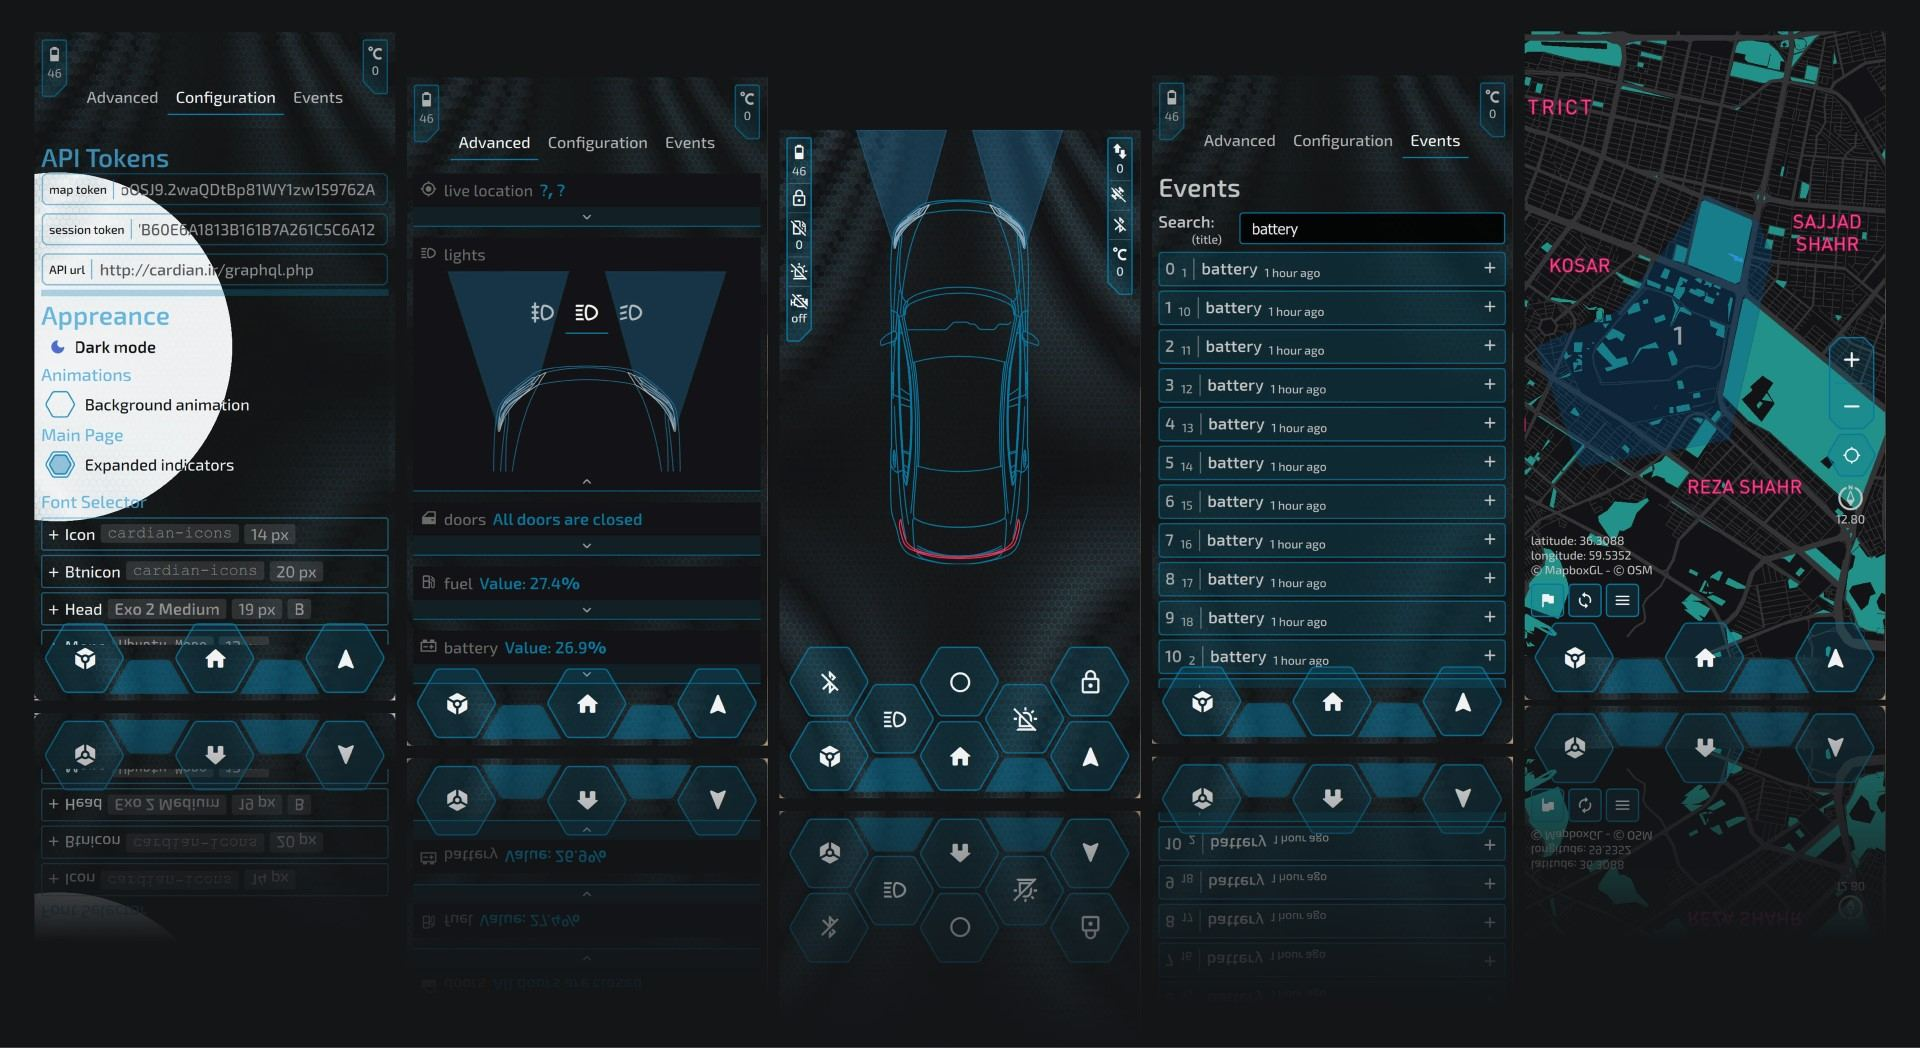
\includegraphics[width=0.7\textwidth]{images/preview-dark.jpeg}
		\caption{حالت تاریک}
		\label{subfig1:fig1:sec2:chap4}
	\end{subfigure}
	\begin{subfigure}[t]{\linewidth}
		\centering
		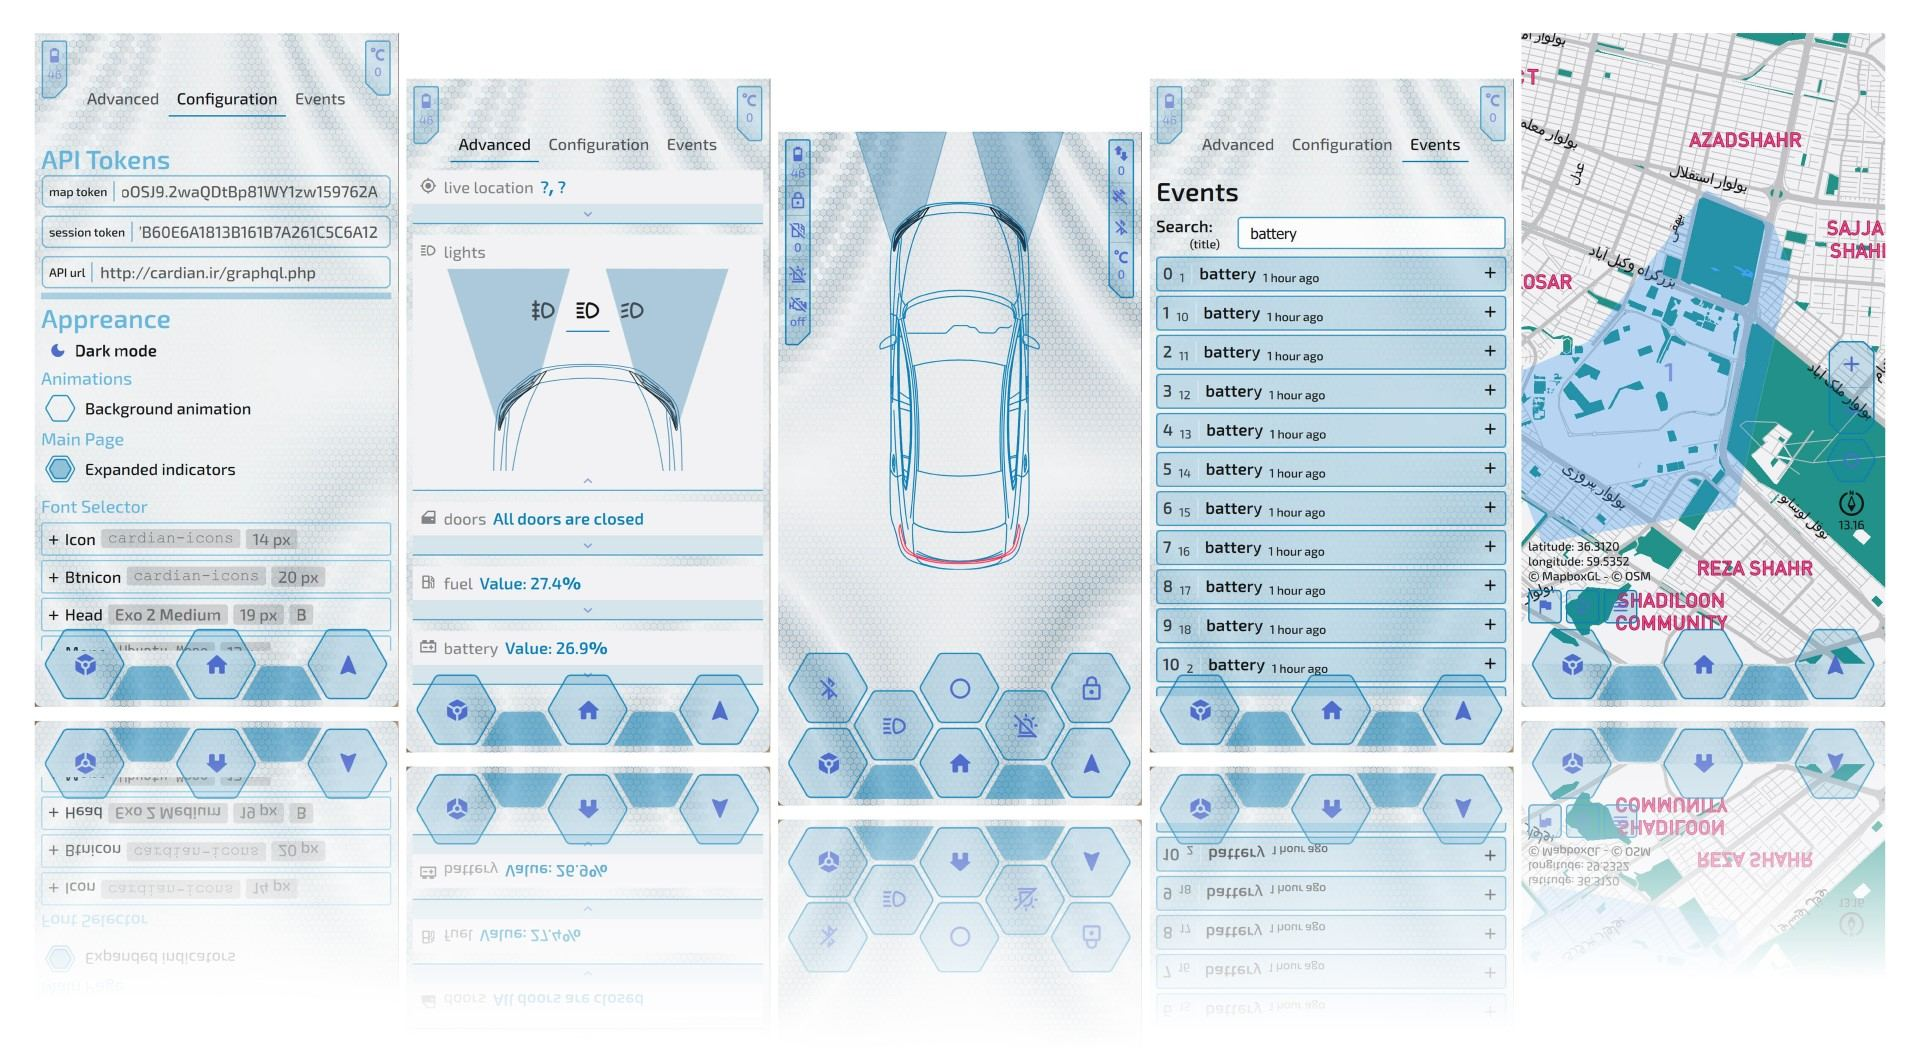
\includegraphics[width=0.7\textwidth]{images/preview-light.jpeg}
		\caption{حالت روشن}
		\label{subfig2:fig1:sec2:chap4}
	\end{subfigure}
	\hspace*{1cm}
	\normalsize
	\label{fig1:sec2:chap4}
	\caption{پیشنمایش‌های برنامهٔ سمت کاربر}
\end{figure}

\section{ساختار برنامهٔ سمت سرور}\label{sec3:chap4}

نقش سرور در پروژه، مطابق با
\hyperref[fig1:sec1:chap4]{دیاگرام معماری پروژه}
 ارتباط بین برنامهٔ سمت کاربر و سخت‌افزار اصلی در خودرو است. که در حال حاضر از زبان پرس‌وجوی \lr{GraphQL} برای ایجاد یک \lr{API} تبادل اطلاعات استفاده شده‌است.

پیاده‌سازی \lr{API} در سمت سرور با استفاده از زبان
\lr{PHP}
انجام شده، علت انتخاب این زبان سادگی و پر استفاده بودن بین مابقی زبان‌ها است. که امکان تهیهٔ
سرویس‌های ارزان‌تر با پشتیبانی پیش فرض از مفسر این زبان تسهیل بخشیده است.


\subsection{زبان برنامه‌نویسی \lr{PHP}}\label{subsec1:sec3:chap4}

یک زبان مفسری همه منظوره و مناسب برای توسعهٔ وب است،‌ این اجازه را به توسعه دهندگان می‌دهد تا بتوانند صفحات پویا و تعاملی وب را طراحی کنند.

\lr{PHP}\LTRfootnote{PHP: Hypertext Preprocessor.}
می‌تواند درون کد‌های \lr{HTML} جاسازی شود،‌با پایگاه‌داده ارتباط برقرار کند.
این زبان متن باز است و شامل گروه‌های بزرگی از برنامه‌نویسان و توسعه‌دهندگان است.

در حال حاضر و در زمان نوشتن این مقاله آخرین نسخهٔ این زبان ۸٫۲ بوده و شامل تغییرات فراوانی نسبت به نسخهٔ پیشین خود یعنی ۷٫۴ داشته است.
\cite{PHPDoc:online}

\subsection{تکنولوژی \lr{GraphQL}}\label{subsec2:sec3:chap4}

\lr{GraphQL}
یک زبان پروس‌وجو برای \lr{API}ها و برای فراهم کردن امکان درخواست\lr{Query}ها است، بدین صورت که اطلاعات کاملی دربارهٔ داده‌های \lr{API} شما به کاربر می‌دهد، و این قدرت را به کاربر می‌دهد تا دقیقاً چیزی رو درخواست کند که نیاز دارد و از هر گونه اطلاعات اضافی صرفه‌نظر شود.

\lr{GraphQL}
با امکان تعریف نوع داده‌ها و تعریف فراهم کننده‌ها در سمت سرور این امکان را فراهم می سازد تا به صورت جزئی برای هر مقدار عملیاتی جدا صورت بگیرد و فقط برای بخش اطلاعاتی که کاربر درخواست کرده پردازش و ارسال اطلاعات صورت بگیرد.

و این امکان را فراهم می‌سازد تا فقط با ارسال یک درخواست تمامی داده‌های مورد نیاز خود را در کمترین حجم داده دریافت کند.

این طریقهٔ ارسال داده کاملاً مناسب با شرایط موجود در ریزپردازنده‌ها و این پروژه است، در حالی که منابع برای پردازش و ارسال چندین درخواست پیاپی موجود نیست و می‌توان با فقط یک درخواست بیشتر داده‌های خواسته شده را بدست آورد.

تکنولوژی \lr{GraphQL} امروزه در مقابل تکنولوژی \lr{SOAP}\footnote{\lr{Simple Object Access Protocol}, یک شیوه‌نامه بر پایهٔ \lr{XML} است.}
 و \lr{REST API} قرار می‌گیرد، و با تسهیل ارسال درخواست و خوانایی بسیار بالا محبوبیت بسیار بالایی در بین توسعه‌دهنده‌ها پیدا کرده‌است.
\cite{GraphQL:online}

	\pagebreak
	\opchapter{تشریح سخت‌افزار}\label{chap5}

همانطور که مشخص است، این پروژه از $3$ بخش \emph{نرم‌افزار}، \emph{سرویس
\lr{API}
	 سرور} و \emph{سخت‌افزار} تشکیل شده‌است، که بخش سخت افزار شامل یک کنترل کنندهٔ از راه دور و قلب پردازشی دزدگیر تشکیل شده است.

در بخش سخت‌افزاری کنترل از راه دور
(\lrm{remote})
از یک ریزپردازندهٔ با معماری \lr{AVR} و سری
\lrm{Atmega32p}
 استفاده شده، که برای سهولت کار در حال حاضر از کتابخانه‌ها و برد آمادهٔ‌ \lr{Arduino} برای راه‌اندازی این بخش استفاده شده.

و در مقابل در سمت سخت‌افزار اصلی پروژه نیز از ریزپردازندهٔ
\lrm{ARM}سری \lrm{STM32f013CBT6} استفاده شده، این بخش مستقیماً
و بدون دخالت هیچ برد توسعه‌ای مورد استفاده قرار گرفته‌است.


\section{\rl{کنترل کنندهٔ} \lr{Remote}}\label{sec1:chap5}

همانطور که گفته شد برای این بخش از برد‌های آمادهٔ \lr{Arduino}
استفاده شده‌است.

\lrm{Arduino Pro Mini} یکی از برد‌های توسعه داده‌شده توسط شرکت \lr{Arduino} است، این برد با هستهٔ \lrm{Atmega32p} شامل مشخصات ذیل است:

\begin{itemize}[nosep]
    \item پردازندهٔ $8$ بیت و فرکانس خارجی $8$ مگاهرتز.
    \item $32$ پایه ورودی و خروجی.
    \item یک \lr{SPI}\LTRfootnote{SPI: Serial Peripheral Interface}.
    \item یک \lr{USART}\LTRfootnote{USART: Universal Synchronous/Asynchronous Receiver Transmitter}.
    \item $6$ خروجی \lr{PWM}\LTRfootnote{PWM: Pulse Width Modulation}.
    \item $2$ وقفهٔ خارجی.
    \item $8$ مبدل آنالوگ به دیجیتال (\lr{ADC}\LTRfootnote{ADC: Analog-to-Digital Converter}).
    \item $32$کیلوبایت فضای \lr{SRAM}\LTRfootnote{SRAM: Static Random Access Memory}.
    \item یک کیلوبایت حافظهٔ \lr{EEPROM}\LTRfootnote{EEPROM: Electrically Erasable Programmable Read-Only Memory}.
\end{itemize}
و دیگر موارد است.
\cite{atmega328p_datasheet}

\begin{figure}[!h]
	\begin{center}
		\includegraphics[width=0.4\textwidth]{images/aTmega328p-pins.pdf}
	\end{center}
	\caption{نمایی از پایه‌های خروجی ریزپردازندهّ \lr{AVR}}
	\label{fig1:sec1:chap1}
\end{figure}

\subsection{ماژول‌های خارجی}\label{subsec1:sec1:chap5}

قطعات استفاده شده شامل یک نمایشگر، فرستنده/گیرندهٔ رادیویی،‌ چند دکمه و خازن هستند.


\subsubsection{فرستندهٔ \lr{RF}}\label{subsubsec2:subsec1:sec1:chap5}

ماژول‌های اضافی مورد استفاده در \lr{remote} شامل فرستندهٔ \lr{RF} مدل \lr{HM-TRP} از شرکت سازندهٔ \lr{HopeRF} است، که طبق مشخصات توضیح داده شده در \lr{datasheet} این محصول، یک ماژول به‌صرفه و مصرف منابع بسیار پایین است، برخی از ویژگی‌های این محصول در ذیل لیست شده:
\cite{hmtrp-datasheet}

\begin{itemize}[nosep]
    \item در اندازهٔ بسیار کوچک $16$ در $20$ در $2$ طراحی شده، و در حالت \lr{DIP} و \lr{SMD} قابل نصب است.
    \item کنترل این ماژول توسط \lr{USART} قابل انجام است و فقط کافی است که داده‌ها به ماژول ارسال شوند.
    \item در این ماژول از مدولاسیون \lr{FSK} و برپایهٔ فرکانس استفاده شده که به نسبت مدولاسیون \lr{ASK} ایمن‌تر است.
    \item ارتباط به صورت نیمه-دوطرفه انجام می‌شود.
    \item مصرف این ماژول بین 40 تا \lr{100mW}قابل تغییر است.
    \item و سرعت انتقال داده نیز از $1.2$\lr{Kbps} تا $115.2$\lr{Kbps} قابل تغییر است.
    \item همچنین طبق ادعای شرکت سازنده، برد فرستندهٔ این ماژول در فضای باز تا حداکثر فاصلهٔ $1.5$ کیلومتر است.
\end{itemize}

در ماژول فوق اتصالات بدین ریز پردازنده بدین صورت میباشند.

\begin{figure}[!h]
	\begin{center}
		\includegraphics[width=0.35\textwidth]{images/hmtrp-connections.pdf}
	\end{center}
	\caption{طریقهٔ اتصال ماژول به ریزپردازنده}
	\label{fig1:sec1:chap1}
\end{figure}

\subsubsection{صفحهٔ نمایش \lr{OLED}}\label{subsubsec3:subsec1:sec1:chap5}

در تعریف
\lr{OLED}\LTRfootnote{Organic Light-Emitting Diode.}
 یک \lr{LED} است که از یک لایهٔ
ترکیب آلی استفاده شده که در اثر یک جریان یا میدان الکتریکی از خود نور ساطع می‌کند.

در این پروژه در سخت‌افزار \lr{remote} برای نمایش اطلاعات خودرو از یک نمایشگر \lr{OLED} از سری
\lrm{ER-OLEDM0.91}
 با اندازهٔ
$128\times32$
  پیکسل استفاده شده‌است.

این نمایشگر دارای ارتباط
\lr{I2C}\LTRfootnote{Inter Integrated Circuit.}
 است و می‌تواند با ولتاژ $3.3$ تا $5.5$ راه‌اندازی شود، همچنین مصرف جریان این ماژول از $23$ تا $27$ میلی آمپر است.

این نمایشگر در دستهٔ
\lr{PMOLED}\LTRfootnote{Active Matrix OLED.}
 قرار می‌گیرد که مصرف بیشتری به نسبت
\lr{AMOLED}\LTRfootnote{Passive Matrix OLED.}
 دارد، اما مصرف نمایشگر‌های \lr{OLED} نسبت نمایشگر‌های \lr{LCD} کمتر هستند.
\cite{OrganicE14:online}

طریقهٔ اتصال پین‌های نمایشگر به
\lr{remote}
به صورت زیر است:

\begin{figure}[!h]
	\begin{center}
		\includegraphics[width=0.35\textwidth]{images/oled-connections.pdf}
	\end{center}
	\caption{طریقهٔ اتصال ماژول \lr{OLED} به پردازنده}
	\label{fig1:sec1:chap5}
\end{figure}

\section{سخت‌افزار اصلی (\lr{Main Board})}\label{sec2:chap5}

سخت‌افزار اصلی شامل ریز پردازندهٔ \lrm{STM32} با معماری \lr{ARM} و از سری \lrm{STM32F103CBT6} است، که مشخصات این ریز پردازنده مطابق ذیل است:

\begin{itemize}[nosep]
    \item دارای سه \lrm{USART}، دو \lrm{SPI}، دو \lrm{I2C}، یک ارتباط \lrm{USB}، یک زمان‌سنج  \lrm{PWM}، و یک ارتباط سخت‌افزاری \lrm{CAN} است.
    \item همچنین دارای $48$ پین (پکیج \lrm{LQFP48}\LTRfootnote{Low-profile Quad Flat Pack 48}).
    \item که $37$ تا از آن‌ها ورودی و خروجی است.
    \item دارای $7$ زمان‌سنج.
    \item $2$ مبدل آنالوگ به دیجیتال سخت‌افزاری (با دقت $12$ بیت).
    \item ولتاژ کاری $2.0$ تا $3.6$.
    \item
    و دمای کاری منفی $40$$\deg$ تا $85$$\deg$ درجهٔ سانتی‌گراد است.
    \item همچنین $64$ کیلوبایت حافظهٔ قابل برنامه‌نویسی \lr{FLASH} و $20$ کیلوبایت حافظهٔ
\lr{SRAM} را داراست.
\end{itemize}

در عکس زیر نیز شمای کلی این ریزپردازنده قابل مشاهده است.

\begin{figure}[!h]
	\begin{center}
		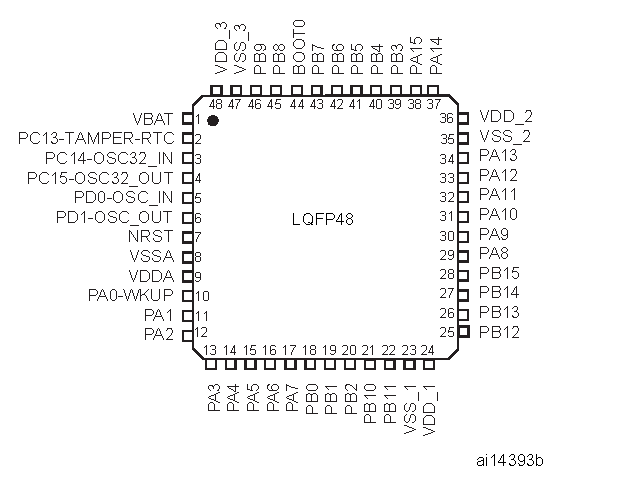
\includegraphics[width=0.6\textwidth]{images/STM32103xx.pdf}
	\end{center}
	\caption{نمایی از پایه‌های خروجی ریزپردازندهّ \lr{STM32F103CBT6}}
	\label{fig1:sec2:chap1}
\end{figure}


دلیل انتخاب این ریزپردازنده قیمت نصب و با امکانات سه برابری نسبت به نسخهٔ
\lrm{ARM}
 هست، همچنین با توجه به تعداد بالای قطعات خارجی نیاز به وجود حداقل $3$
\lrm{USART}
 سخت‌افزاری است، که در این ریزپردازنده فراهم شده است.

\subsection{ماژول‌های خارجی}\label{subsec1:sec2:chap5}

در این بخش از پروژه از ماژول‌های \lr{GPS}، ماژول \lr{GSM}،‌ فرستنده/گیرندهٔ رادیویی،
چند رله، ماسفت و دیگر قطعات استفاده شده است.


\subsubsection{ماژول \lr{GPS}}\label{subsubsec1:subsec1:sec2:chap5}

ماژول \lr{GPS} در این پروژه برای موقعیت یابی استفاده شده است، این ماژول از سری \lrm{neo6mv2} و ساختهٔ شرکت \lr{ublox} است.

ارتباط با این ماژول از طریق \lr{USART} صورت می‌گیرد که در صورت اتصال موفق به ماهواره، به صورت پیاپی و در هر ثانیهٔ اطلاعات مربوط به موقعیت از طریق \lr{USART} به پردازنده ارسال می‌شود.

این اطلاعات شامل موقعیت جغرافیایی، فاصله از سطح دریا، تعداد ماهواره‌های در دسترس، سرعت، زمان در فرمت \lr{UTC} و موارد دیگر است، که در زیر دسته‌های این اطلاعات لیست شده است:

\begin{itemize}[nosep]
    \item \lrm{\$GPGSA}: اطلاعات مربوط به ماهواره‌های فعال.
    \item \lrm{\$GPGSV}: ریز اطلاعات مربوط به ماهوارهٔ \lr{GPS}.
    \item \lrm{\$GPGLL}: اطلاعات جغرافیایی از جمله عرض و طول جغرافیایی.
    \item \lrm{\$GPRMC}: اطلاعات ضروری مانند سرعت، زمان، و شتاب.
    \item \lrm{\$GPVTG}: اطلاعات مربوط به جهت حرکت، و سرعت زمان.
\end{itemize}

در اینجا فقط از اطلاعات در خط \lr{GPGGA} استفاده شده است که خلاصهٔ اطلاعات ضروری \lr{GPS} است، این اطلاعات با مقدار \lr{\$GPGGA} شروع شده و سپس به دنبال آن $14$ فیلد دادهٔ دیگر جدا شده توسط «,» (\lr{comma}) قرار گرفته‌اند، این اطلاعات به ترتیب شامل لیست

\textit{
\hypersetup{linkcolor=gray}
\hyperref[i1:enum1:sec2:chap5]{utc},
\hyperref[i2:enum1:sec2:chap5]{latitude},
\hyperref[i3:enum1:sec2:chap5]{N},
\hyperref[i4:enum1:sec2:chap5]{Longitude},
\hyperref[i5:enum1:sec2:chap5]{W},
\hyperref[i6:enum1:sec2:chap5]{quality-code},
\hyperref[i7:enum1:sec2:chap5]{satellites-num},
\hyperref[i8:enum1:sec2:chap5]{horizontal-dilution},
\hyperref[i9:enum1:sec2:chap5]{altitude},
\hyperref[i10:enum1:sec2:chap5]{M},
\hyperref[i11:enum1:sec2:chap5]{mean-sea-level},
\hyperref[i12:enum1:sec2:chap5]{M},
\hyperref[i13:enum1:sec2:chap5]{last-DGPS-UTC \textbar{} dgps-station-id},
\hyperref[i14:enum1:sec2:chap5]{checksum}
}
است.
\begin{enumerate}[nosep]
    \item \label{i1:enum1:sec2:chap5}\lr{UTC} زمان اتصال به ماهواره و ثابت شدن در میلی‌ثانیه.
    \item \label{i2:enum1:sec2:chap5}\lr{latitude} عرض جغرافیایی.
    \item \label{i3:enum1:sec2:chap5}\lr{N} علامت جهت شما یا جنوب.
    \item \label{i4:enum1:sec2:chap5}\lr{longitude} طول جغرافیایی.
    \item \label{i5:enum1:sec2:chap5}\lr{W} علامت جهت غرب با شرق.
    \item \label{i6:enum1:sec2:chap5}\lr{quality-code} کد ثبات \lr{GPS}: \lrm{0} (نا معتبر)، \lrm{1} (ثبات \lr{GPS}), \lrm{2} (ثبات \lr{DGPS}), \lrm{3}
    (ثبات \lr{PPS}) , \lrm{4} (بی‌درنگ), \lrm{5} (\lr{Float RTK}), \lrm{6} (تقریبی), \lrm{7} (ورودی دستی), \lrm{8}
    (حالت شبیه‌سازی)
    \item \label{i7:enum1:sec2:chap5}\lr{satellites-num} تعداد ماهواره‌های تشخیص داده شده.
    \item \label{i8:enum1:sec2:chap5}\lr{horizontal-dilution} اندازه گیری کیفیت هندسی ماهواره های \lr{GPS} در دید.
    \item \label{i9:enum1:sec2:chap5}\lr{altitude} ارتفاع از سطح دریا.
    \item \label{i10:enum1:sec2:chap5}\lr{M} واحد ارتفاع.
    \item \label{i11:enum1:sec2:chap5}\lr{mean-sea-level} تفاوت ارتفاع بین بیضی مرجع \lr{WGS84} و ژئوئید زمین.
    \item \label{i12:enum1:sec2:chap5}\lr{M} واحد ارتفاع.
    \item \label{i13:enum1:sec2:chap5}\lr{last-DGPS-UTC} --زمان از آخرین بروز رسانی \lr{DGPS. DGPS-station-id -- DGPS station ID number }
    \item \label{i14:enum1:sec2:chap5}*42 -- دادهٔ تشخیص صحت مقدار، همیشه با \lrm{*} شروع می‌شود.
\end{enumerate}

در اینجا اطلاعات در پردازندهٔ \lr{STM32} دریافت شده و مقادیر توسط «,» جدا می‌شوند، سپس به صورت یک ساختار در یک \lr{ring-buffer} ذخیره می‌شوند.

در مقابل این ماژول، ماژول‌های سری \lr{L} از شرکت \lr{Quectel} قرار می‌گیرند که به ظاهر کیفیت بهتری دارند، اما به نسبت قیمت ماژول‌های شرکت \lr{ublox} مقرون به‌صرفه‌تر هستند.
\cite{GPVTG21:online}

\subsubsection{ماژول \lr{SIM800L}}\label{subsubsec2:subsec1:sec2:chap5}

برای ارسال داده‌ها به سمت سرور نیاز به اتصال به اینترنت است که این اتصال به واسطهٔ ماژول‌های سیم‌کارت صورت می گیرد.

از جمله ماژول‌های بیشتر مورد استفاده شده ماژول \lrm{SIM800L} است که ارزان‌ترین ماژول \lr{GSM} از شرکت \lr{SimCom} است، ماژول \lrm{SIM800L} امکان برقراری ارتباط به صورت \lr{2G} را فراهم می‌کند.

این ماژول همچنین قابلیت ارسال و دریافت پیام‌کوتاه، ارسال ایمیل، ایجاد تماس صوتی، ارسال \lr{MMS}، ضبط صوت، ایجاد ارتباط \lr{FTP}، ایجاد درخواست \lr{HTTP} و دیگر موارد را داراست.

تقریباً در اکثر نقاط کشور امکان ارتباط به صورت \lr{2G} فراهم شده‌است، پس یکی به‌صرفه ترین راه‌ها برای اتصال به سرور استفاده از ماژول‌های سیم‌کارت است.

همچنین از راه‌های دیگر ارتباط اینترنتی در نقاط مختلف، می‌‌توان به ارتباط‌های ماهواره‌ای از طریق ماژول‌های \lr{LORA} و \lr{Swarm} از شرکت \lr{Space X} اشاره کرد که راه‌حلی جدید برای اینترنت‌اشیاء در تمامی نقاط است، اما به نسبت هزینه در مقابل \lr{SIM800L} به‌صرفه نیست.

این ماژول از ارتباط \lr{USART} برای ارسال و دریافت داده‌ها به پردازنده استفاده می‌کند، و دستورات به صورت مجموعه‌ای از \lr{AT-Command}ها به ماژول ارسال می شوند.

ماژول‌های \lr{SIM800} دارای پیچیدگی بسیار بالایی هستند و یک محدودهٔ‌ بزرگی از امکانات را در اختیار توسعه‌دهنده قرار می‌دهند، و طبق ادعای شرکت \lr{SimCOM} تمامی قابلیت‌های یک تلفن هوشمند و یا یک کامپیوتر شخصی را به شما می‌دهند.

در ادامهٔ مشخصات ماژول \lr{SIM800L}، این ماژول نیاز به توان ورودی بین $3.4$ تا $4.4$ ولت را نیاز دارد. این ماژول در حالت خواب (\lr{sleep mode}) فقط $0.7$
میلی‌آمپر توان مصرف می‌کند. این ماژول همچنین از $4$ باند فرکانس‌های \lr{GSM} پشتیبانی می‌کند، که توان ارسال آن وابسته به باند فرکانس تنظیم شده است.
همچنین دمای کاری ماژول بین منفی $40$ تا $85$ درجهٔ سانتیگراد است.

ارسال داده‌های \lr{GPRS} نیز می‌تواند تا حداکثر سرعت $85$\lr{Kbps} انجام پذیرد. ماژول از قابلیت‌ \lr{USSD} پشتیبانی می‌کند و همچنین دارای پشتیبانی از نسخه‌های سیم‌کارت $1.8$ تا نسخهٔ $3$ است.

می‌توان برای تقویت ماژول از یک آنتن خارجی استفاده کرد. این ماژول در بخش صورت دارای قابلیت های رفع نویز و رفع اکو نیز است. و دارای قابلیت \lr{Real time} است که همچنین قابل فعال‌سازی است.

اندازهٔ ماژول در \lr{15.8x17.8x2.4mm} است و دارای وزن $1.35$ گرم است.
\cite{sim800}

\paragraph{طریقهٔ اتصال}\label{par1:subsubsec1:subsec1:sec2:chap5}

بر روی ماژول‌های موجود در بازای یک محافظ فلزی برای جلوگیری از آسیب دیدگی و رفع نویز قرار داده شده، که همچنین برای استفادهٔ راحت‌تر عموماً توسط یک مبدل \lr{DIP} به فروش می‌رسند که تا $12$ پین از آن در دسترس است.
پین‌های خروجی ماژول به صورت زیر هستند:

\begin{figure}[!h]
	\begin{center}
		\includegraphics[width=0.3\textwidth]{images/sim800-pins.pdf}
	\end{center}
	\caption{پین‌های خروجی در ماژول \lr{SIM800L}}
	\label{fig1:sec2:chap5}
\end{figure}

\LTRfootnotetext{DTR: Data Ready.}
\LTRfootnotetext{GND: Ground.}
\LTRfootnotetext{MIC: Microphone.}
\LTRfootnotetext{Net: Antena.}
\LTRfootnotetext{RING: Phone Ring.}
\LTRfootnotetext{RST: Reset.}
\LTRfootnotetext{RXD: UART data reciver.}
\LTRfootnotetext{SPK: Speaker.}
\LTRfootnotetext{TXD: UART data transmiter.}

در کنار این توضیحات،‌ استفاده از این ماژول نیازمند کمی دانش اولیه برای راه‌اندازی آن است، که این نکات عبارت‌اند از:

\begin{enumerate}[nosep]
    \item بهتر است ورودی توان ماژول مقدار $4.4$ ولت باشد، هر مقداری بیش‌از این موجب سوختن ماژول خواهد شد. همچنین جریان ورودی مورد نیاز در حالت مناسب باید تا $2$ آمپر باشد.
    \item برای استفاده از مآژول توصیه شده که از ولتاژ $3.3$ برای ورودی \lr{TX}استفاده شود. این کار می تواند با قراردهی یک دیود در بین پایه‌های \lr{TX} و \lr{RX} انجام شود.
    \item برای بررسی فعال بودن یا نبودن ماژول می‌توان پین \lr{Ring} را بررسی کرد، که باید همیشه مقدار آن $4$ ولت باشد.
    \item برای تشخیص راه‌اندازی مجدد شدن ماژول می‌توان گزینه‌های زیر را برررسی کرد،
    در صورت راه‌اندازی مجدد به احتمال زیاد توان کافی به ماژول نمی‌رسد و باید این مشکل رفع گردد:

    \begin{enumerate}[nosep]
        \item نشانگر \lr{LED} وضعیت ماژول به سرعت چشمک زده، متوقف شود و سپس مجدداً به چشمک زدن ادامه پیدا کند. بدین معنی که ماژول در اتصال به شبکه مشکل داشته و توان کافی به ماژول نرسیده، پس ماژول شروع به راه‌اندازی مجدد می‌کند.
        \item اگر مقدار پین \lr{Ring} صفر شد.
        \item در صورت ارسال شدن مقدار نال (\lr{Null}) از طریق \lr{USART}.
        \item مشاهدهٔ مقدار \lrm{SMS\ Ready}یا \lrm{Call\ Ready} بعد از هر دستور.
    \end{enumerate}
    \item ماژول‌های \lr{SIM800} برای اتصال به شبکه نیازمند جریان لحظه‌ای $2$ آمپر هستند،
    که عموماً فراهم کردن تغذیه‌ای با خروجی $2$ آمپر ممکن نیست، برای رفع این مشکل می‌توان از یک خازن $1500$\lr{uF} در بین پایه‌های زمین و $4$ ولت استفاده کرد.
    همچنین استفاده از خازن‌های پلیمری برای اینکار توصیه می‌شوند.
\end{enumerate}


\paragraph{دستورات}\label{par2:subsubsec1:subsec1:sec2:chap5}

برخی از دستورات مهم ماژول به شرح زیر هستند:

\begin{enumerate}[nosep]
    \item \lrm{ATA}: پاسخ تماس.
    \item \lrm{ATZ}: بازنشانی تنظیمات پیشفرض.
    \item \lrm{ATI}: اطلاعات ماژول.
    \item \lrm{ATD+980123456789;}: ایجاد تماس.
    \item \lrm{ATH}:پایان تماس.
    \item \lrm{AT\&F}: تنظیمات کارخانه.
    \item \lrm{AT\&V}: نمایش تنظیمات فعلی.
    \item \lrm{AT\&W}: ذخیرهٔ نمایهٔ فعال.
    \item \lrm{AT+HVOIC}: قطع فقط تماس.
    \item \lrm{AT+CPOWD=1}: خاموش کردن ماژول.
    \item \lrm{AT+CPOWD=0}: خاموش کردن فوری.
    \item \lrm{AT+SJDR=\textless{}n\textgreater{}}: تنظیم تشخیص اختلال.
    \item \lrm{AT+CANT=1,0,10}: فعال‌سازی تشخیص آنتن.
    \item \lrm{AT+CANT=1,1,10}: فعال‌سازی تشخیص آنتن و اطلاع رسانی آن هر $10$
    ثانیه.
    \item \lrm{AT+CROAMING}: حالت رومینگ.
    \item \lrm{AT+CBATCHK=1}: تنظیم ولتاژ پشتیبانی.
    \item \lrm{AT+CPAS}: گزارش وضعیت ماژول.
    \item \lrm{AT+CSQ}: گزارش کیفیت سیگنال.
    \item \lrm{AT+CFUN=1}: تنظیم عملکرد ماژول.
    \item \lrm{AT+CFUN=1,1}: راه‌اندازی مجدد و تنظیم عملکرد کامل ماژول.
    \item \lrm{AT+CCLK?}: ساعت.
    \item \lrm{AT+CBC}: میزان باتری.
    \item \lrm{AT+CSCLK?}: فعال‌سازی حالت آهسته.
    \item \lrm{AT+CSCLK=0}: غیر فعال‌سازی حالت آهسته.
    \item \lrm{AT+CENG}: تغییر به حالت مهندسی.
\end{enumerate}

\paragraph{\lr{GPRS}}\label{par3:subsubsec1:subsec1:sec2:chap5}
\begin{enumerate}[nosep]
    \item \lrm{AT+CGATT=1}: اتصال یا قطع ارتباط \lr{GPRS}.
    \item \lrm{AT+SAPBR=3,1,"Contype","GPRS"}: تنظیم نوع اتصال \lr{GPRS}.
    \item \lrm{AT+SAPBR=3,1,"APN","mtnirancell"}: تنظیم مقدار \lr{APN} اپراتور.
    \item \lrm{AT+SAPBR=1,1}: فعال‌سازی \lr{GPRS}.
    \item \lrm{AT+SAPBR=0,1}: قطع \lr{GPRS}.
    \item \lrm{AT+SAPBR=2,1}: گرفتن مقدار \lr{IP}.
\end{enumerate}

\paragraph{دستورات آمادهٔ پیاپی}\label{par4:subsubsec1:subsec1:sec2:chap5}

در زیر لیستی از دستورات و روال‌ها برای انجام برخی عملیات ضروری‌تر توسط ماژول فراهم شده است.
باید توجه کرد که اجرای دستورات باید به صورت سری و پشت سر هم و با وقفهٔ بسیار کم باشند.
همچنین اجرای هر دستور نیازمند فعال‌سازی دستورات قبل است.

\subparagraph{\rl{راه‌اندازی مجدد}}\label{subpar1:par4:subsubsec1:subsec1:sec2:chap5}
\:\newline\:
\begin{latin}
	\small
	\begin{lstlisting}[language=bash,caption={restarting module}]
        # Airplane mode
        AT+CFUN=0
		# Full function
		AT+CFUN=1
	\end{lstlisting}
\end{latin}

\subparagraph{\rl{فعال‌سازی} \lr{GPRS}}\label{subpar2:par1:subsubsec1:subsec1:sec2:chap5}
\:\newline\:
\begin{latin}
	\small
	\begin{lstlisting}[language=bash,caption={Enable GPRS}]
		# AT+SAPBR=<type>,<cid>[,<param>,<value>]
		# <type>: 0.close 1.open 2.open 3.set parameter
		# Set connection type
		AT+SAPBR=3,1,"Contype","GPRS"
		# Set APN(Access Point Name)
		AT+SAPBR=3,1,"APN","mtnirancell"
		# Enable GPRS, Open bearer
		AT+SAPBR=1,1
		# Query bearer
		AT+SAPBR=2,1
	\end{lstlisting}
\end{latin}

\subparagraph{\rl{غیرفعال‌سازی} \lr{GPRS}}\label{subpar3:par1:subsubsec1:subsec1:sec2:chap5}
\:\newline\:
\begin{latin}
	\small
	\begin{lstlisting}[language=bash,caption={Disabling GPRS}]
		# Disable GPRS
		AT+SAPBR=0,1
	\end{lstlisting}
\end{latin}

\subparagraph{\rl{درخواست} \lr{HTTP}}\label{subpar4:par1:subsubsec1:subsec1:sec2:chap5}
\:\newline\:
درخواست‌های \lr{Http} در ماژول \lr{SIM800} بعد از فعال‌سازی \lr{GPRS} ممکن است، اما احتمال موفقیت ارسال این درخواست نسبت به ایجاد ارتباط خام \lr{TCP} کمتر است،
به این دلیل که تعداد دستورات بیشتر بوده و متأسفانه رابط استفاده از دستورات به هیچ عنوان مناسب نیست، و استفاده از این رابط به شدت مشکل است.

پس در این پروژه مستقیماً درخواست‌ها به صورت درخواست خام \lr{TCP} ارسال شده‌اند.

\begin{latin}
	\small
	\begin{lstlisting}[language=bash,caption={HTTP request}]
		# Initialize
		AT+HTTPINIT

		# Add Http params
		# AT+HTTPPARA=<param name>,<value>
		# AT+HTTPPARA="CID",<profile-id>
		AT+HTTPPARA="CID",1

		# AT+HTTPPARA="URL",<target url>
		AT+HTTPPARA="URL","http://cardian.ir/graphql"

		# Set Http content-type
		# AT+HTTPPARA="CONTENT","<mime types>"
		AT+HTTPPARA="CONTENT","application/json"

		# AT+HTTPDATA=<data size>,<wait in ms>
		AT+HTTPDATA=192,5000

		# Post DATA, if there is a post
		postdata

		# AT+HTTPACTION=<action>
		# <action>:0 GET, 1 POST, 2 HEAD, 3 DELETE
		AT+HTTPACTION=0

		# Read all data
		AT+HTTPREAD

		# Terminate HTTP Service
		AT+HTTPTERM
	\end{lstlisting}
\end{latin}

\subparagraph{\rl{ایجاد ارتباط} \lr{TCP}}\label{subpar5:par1:subsubsec1:subsec1:sec2:chap5}
\:\newline\:
\begin{latin}
	\small
	\begin{lstlisting}[language=bash,caption={TCP connection}]
		# set to single connection
		AT+CIPMUX=0
		# Set default APN
		AT+CSTT="mtnirancell","",""
		# Start wireless connection
		AT+CIICR
		# Get assigned IP address
		AT+CIFSR

		# Close old connections (optional)
		# $ SHUT OK
		AT+CIPSHUT
		# manually read data (optional)
		AT+CIPRXGET=1
		# AT+CIPSTART="<TCP/UDP>","<server>","<port>"
		AT+CIPSTART="TCP","cardian.ir",80
		# Send TCP packet
		# AT+CIPSEND=<data-length>
		AT+CIPSEND=107

		POST /index.html HTTP/1.0\nHOST: cardian.ir\nContent-type: application/json\nContent-length: 13\n{"test":true}\n

		# Close TCP connection
		AT+CIPCLOSE
	\end{lstlisting}
\end{latin}

\emph{\textbf{نکته}: در صورتی که مقدار \lrm{+PDP:\ DEACT\ URC} توسط ماژول گزارش شد به معنی جداسازی و قطع شدن \lrm{GPRS} توسط شبکه است. در این حالت کاربر باید دستور \lrm{AT+CIPSHUT} را برای تغییر زمینهٔ
\lrm{PDP} به حالت اصلی انجام دهد. در غیر این صورت امکان اتصال مجدد \lr{GPRS} به شبکه نیست.}
\cite{sim800}

\section{طراحی شماتیک و فیبر مدار چاپی}\label{sec3:chap5}
برای طراحی شماتیک \footnote{یک نمایش گرافیکی است که از اجزاء مختلف یک مدار الکتریکی و اتصالات بین آن‌ها تشکیل شده‌است.}
 مدار از برنامهٔ
\lr{Altium Designer}\LTRfootnote{\url{https://www.altium.com}}
استفاده شده‌است.

در این پروژه طراحی شماتیک برای بخش‌های مدار اصلی و کنترل انجام شده‌است.

\subsection{برد اصلی}\label{subsec1:sec3:chap5}
طراحی شماتیک مدار اصلی در زیر آمده‌است.
\begin{figure}[!h]
	\begin{center}
		\includegraphics[width=0.8\textwidth]{images/main-hardware-schematic.pdf}
	\end{center}
	\caption{شماتیک مدار اصلی}
	\label{fig1:sec3:chap5}
\end{figure}

\begin{figure}[!h]
	\centering
	\footnotesize
	\begin{subfigure}[t]{0.50\linewidth}
		\centering
		\includegraphics[width=\textwidth]{images/pcb-top-layer.pdf}
		\caption{لایهٔ بالایی}
		\label{subfig1:fig2:sec3:chap5}
	\end{subfigure}
	\begin{subfigure}[t]{0.44\linewidth}
		\centering
		\includegraphics[width=\textwidth]{images/3d-preview.jpg}
		\caption{پیش‌نمایش سه بعدی}
		\label{subfig2:fig2:sec3:chap5}
	\end{subfigure}
	\normalsize
	\label{fig2:sec3:chap5}
	\caption{فیبر مدار چاپی}
\end{figure}

قطعات استفاده شده در شماتیک مطابق لیست زیر است:

\begin{enumerate}[nosep]
	\item \lrm{1x3 Pin Header}.
	\item \lrm{STM32F103CBT6}.
	\item \lrm{SIM800L}.
	\item \lrm{Nano SIM Connector}.
	\item \lrm{NEO-M6-V2 GPS}.
	\item \lrm{HM-TRP 433MHz}.
	\item \lrm{Crystal-XL7KI-111-32M}.
	\item
	\lrm{1206-SMD-Capacitor}:
	\lrm{8pF} ($2$)،
	\lrm{15uf} ($4$).
	\item \lrm{Tantalium Capacitor}.
	\item \lrm{IPEX-MHF1} ($2$).
	\item \lrm{LU-3H Relay} ($6$).
	\item \lrm{SHT20 Temperature Sensor}.
	\item \lrm{1206 SMD LED} ($5$).
	\item \lrm{1206 SMD Resistor}:
	\lrm{10} ($1$)،
	\lrm{1K} ($8$)،
	\lrm{330} ($6$)\footnote{برای استفاده به همراه \lr{LED}ها.}.
	\item \lrm{PHD45N03LTA Mosfet}.
	\item \lrm{3x6 SMD Tacticle Switch}.
	\item \lrm{3.3 Linear Regulator SOT-223}.
\end{enumerate}

	\pagebreak
	\opchapter{پیوست‌ها}

این فصل شامل بخشی از کد‌های نوشته شده به همراه توضیحاتی از آن‌ها است.
مطابق توضیحات در فصل‌های قبلی، پروژه شامل سه بخش بوده که در مجموع از ۶ تا ۷ زبان برنامه‌نویسی مجزا تشکیل شده.
سعی بر اینست که هر بخش به صورت شفاف توضیح داده شود.
\section{نرم‌افزار}
\subsection{درخواست \lr{Post} کلاس \lr{C++}}
فایل اصلی:
\hyperref{https://github.com/cardianco/cardian/blob/master/cardian/requesthandler.h}{}{}{\lrm{cardian/requesthandler.h}}

مورد استفاده: ‌ارسال درخواست‌های \lr{post}.
\begin{latin}
	\small
	\begin{lstlisting}[language=C++, caption={C++ Request Handler Component}]
		/// Implementation details of the main code.
		class requestHandler : public QObject {
			Q_OBJECT
			QML_NAMED_ELEMENT(RequestHandler)
			QML_ADDED_IN_MINOR_VERSION(1)
		public:
			Q_INVOKABLE int postRequest(const QUrl &url, const QByteArray &body, const QVariantMap &extraHeads = QVariantMap(), int timeout = DefaultTransferTimeoutConstant) {
				QNetworkRequest req(url);
				req.setTransferTimeout(timeout);
				req.setHeader(QNetworkRequest::ContentTypeHeader, "application/json");

				for(const auto &head: core::QKVRange(extraHeads)) {
					req.setRawHeader(head.first.toLatin1(), extraHeads[head.first].toByteArray());
				}

				QNetworkReply *reply = mNetworkManager.post(req, body);
				mRequestHash[reply].id = ++mNum;

				emit runningChanged();

				QObject::connect(reply, &QNetworkReply::readyRead, this, &requestHandler::onReadyRead);
				QObject::connect(reply, &QNetworkReply::finished, this, &requestHandler::onFinished);
				QObject::connect(reply, &QNetworkReply::errorOccurred, this, &requestHandler::onErrorOccurred);

				return mNum;
			}

		private:
			QNetworkAccessManager mNetworkManager;
			QHash<QNetworkReply *, replyData> mRequestHash; // The container used for holding each request
			int mNum; /// This is only for counting requests.
		};
	\end{lstlisting}
\end{latin}

\subsection{کلاس \lr{secureKeyChain}}
مورد استفاده: ذخیرهٔ ایمن \lr{token}های کاربر توسط در \lr{keychain}.

آدرس فایل:
\hyperref{https://github.com/cardianco/cardian/blob/master/cardian/securekeychain.h}{}{}{\lrm{cardian/securekeychain.h}}
\begin{latin}
	\small
	\begin{lstlisting}[language=C++, caption={C++ KeyChain Component}]
		/// Implementation details of the main code.
		class secureKeyChain: public QObject, public QQmlParserStatus {
			Q_OBJECT
			Q_PROPERTY(QVariantMap cache READ cache NOTIFY cacheChanged FINAL)

			QML_NAMED_ELEMENT(SecureKeyChain)
			QML_ADDED_IN_MINOR_VERSION(1)
		public:
   			QVariant readKey(const QString &key) {
				if(mCache.contains(key)) return mCache[key];

				credentialReader *reader = new credentialReader(service, this);
				connect(reader, &credentialReader::finished, this, &secureKeyChain::readerFinished);

				reader->setKey(key);
				reader->setAutoDelete(true);
				reader->start();

				return QVariant{}; /// Return undefined
			}
		private:
			QVariantMap mCache;
		};
	\end{lstlisting}
\end{latin}

\subsection{کلاس \lr{ٰVeqtor}}
مورد استفاده: کلاس پایهٔ استفاده شده برای نمایش و رسم شکل‌ها و چارت‌ها.

آدرس فایل:
\hyperref{https://github.com/0smr/veqtor/veqtor.h}{}{}{\lrm{cardian/third-parties/veqtor/veqtor.h}}
\begin{latin}
	\small
	\begin{lstlisting}[language=C++, caption={C++ ٰVeqtor Root Class}]
		/// Implementation details of the main code.
		class veqtor : public QNanoQuickItem {
			Q_OBJECT
			QML_NAMED_ELEMENT(Veqtor)
			QML_ADDED_IN_MINOR_VERSION(1)

			Q_PROPERTY(QString src READ src WRITE setSrc NOTIFY srcChanged)
			Q_PROPERTY(QVariantMap document READ document NOTIFY documentChanged)
			Q_PROPERTY(QObject* root READ root NOTIFY rootChanged)
			Q_PROPERTY(QSizeF sourceSize READ sourceSize CONSTANT)
		public:
			veqtor(QQuickItem *parent = nullptr);
			QNanoQuickItemPainter *createItemPainter() const override final;

			void hoverMoveEvent(QHoverEvent* event) override;

			void componentComplete() override;
			void painter(QNanoPainter *painter) const;

			QPointer<elements::svg> root() { return mRoot; }

			QString src() const { return mSrc; }
			void setSrc(const QString& src);

			QVariantMap document() const { return mDocument; }

			Q_INVOKABLE QVariant getElementById(const QString &id) { return mDocument[id]; }

			QSizeF sourceSize() const { return mSourceSize; }

		private slots:
			void setElementsToProperties();
			void adjustSize();
			void adjustResponsive();
			void updateDocument(const QString &newId, const QString &oldId);
			void updateElementAttributes();

		public slots:
			void update();

		signals:
			void srcChanged();
			void rootChanged();
			void documentChanged();
			void svgLoaded();
			void hovered(QPointer<elements::element> target);

		private:
			QPointer<elements::svg> mRoot;
			QVariantMap mDocument;
			QString mSrc;
			QSizeF mSourceSize;

			QTimer mUpdateTimer;
			QTransform mAdjustment;
		};
	\end{lstlisting}
\end{latin}

\subsection{فایل \lr{Statuses}}
مورد استفاده: نگهداری، و دریافت داده‌ها از سرور.

آدرس فایل:
\hyperref{https://github.com/cardianco/cardian/blob/master/cardian/globals/Status.qml}{}{}{\lrm{cardian/globals/Status.qml}}
\begin{latin}
	\small
	\begin{lstlisting}[language=qml, caption={Global Status Component}]
		/// Implementation details of the main code.
  		RequestHandler {
			id: requestHandler
			property var responses: Object();

			function graphAPI(body) {
				// Config.api == https://cardianWebsite/graphQL.php
				// Config.token == <64 byte hex string> == SHA256
				return postRequest(Config.api, JSON.stringify(body), {stoken: Config.token})
			}

			onErrorOccurred: /* Handling errors */;
			onFinished: function(data, id) {
				if(typeof responses[id].callback == 'function') {
					const args = responses[id].args ?? [];
					responses[id].callback(data, ...args);
					delete responses[id];
				}
			}
		}

		function fetchStatuses() {
			const limit = 100, start = events.first() ?? {};
			const body = { query: `query{statusHistory(limit:${limit},start:${start.id ?? -1}){id fieldType{id name} data utc}}` };
			const id = requestHandler.graphAPI(body);

			reqHndlr.responses[id] = {
				callback: result => {
					const history = JsUtils.parseJson(result, {}).qget('data.statusHistory', []);
					if(history) {
						history.forEach(record => {
							const {id, fieldType, data, utc} = record;
							/// Here, `events` refers to an object instance of `EventModel`.
							events.append(id, fieldType.name, data, utc, fieldType.id);
						});
					}
				}
			};
		}
	\end{lstlisting}
\end{latin}


\subsection{صفحهٔ پیمایش}
مورد استفاده: بخشی از کد صفحهٔ‌ پیمایش نرم‌افزار.

آدرس فایل:
\hyperref{https://github.com/cardianco/cardian/blob/master/cardian/pages/NavigationPage.qml}{}{}{\lrm{cardian/pages/NavigationPage.qml}}
\begin{latin}
	\small
	\begin{lstlisting}[language=qml, caption={Navigation Page}]
		/// Implementation details of the main code.
		RouteModel {
			id: routeModel

			autoUpdate: true
			query: routeQuery

			plugin: Plugin {
				name: "mapbox"
				/// `control.token` here refered as mapboxGL access token.
				PluginParameter { name: "mapbox.access_token"; value: control.token }
			}
		}

		RouteQuery { id: routeQuery }

		contentItem: Map {
			id: map

			opacity: 1.0
			zoomLevel: 14
			copyrightsVisible: false
			center: QtPositioning.coordinate(36.3162, 59.5408) // Mashhad (Default location, clould also be Tehran)
			color: "transparent"
			gesture.enabled: !dragPoly.dragging

			plugin: Plugin {
				name: 'mapboxgl'
				locales: ['en_US' ,'fa_IR']
				preferred: ["mapboxgl", 'osm', "mapbox"]

				PluginParameter {
					name: 'mapboxgl.access_token'
					value: control.token
				}

				PluginParameter {
					name: 'mapboxgl.mapping.cache.memory'
					value: false
				}

				PluginParameter {
					name: 'mapboxgl.mapping.additional_style_urls'
					value: 'qrc:/resources/mapgl/dark-style.json'
				}
			}

			TapHandler {
				id: tapInserter
				grabPermissions: TapHandler.ApprovesTakeOverByAnything
				onTapped: event => {
					const {longitude, latitude} = map.toCoordinate(event.position);
					const {i} = JsUtils.findNearestPoint(Qt.vector2d(longitude, latitude), activePolygon);
					activePolygon.insert(i, {longitude, latitude});
				}
			}

			MapItemView {
				model: routeModel

				delegate: MapRoute {
					route: model.routeData
					line.color: "#aaF5478D"
					line.width: map.zoomLevel > 5 ? map.zoomLevel/2.8 : 0
					smooth: true
					opacity: index ? 0.3 : 1.0
				}
			}

			MapItemView {
				model: polygons

				delegate: MapItemGroup {
					required property int index
					required property var poly

					MapPolygon {
						opacity: 0.3
						color: index === Config.selectedMap ? control.palette.text : control.palette.highlight
						border.color: control.palette.window
						border.width: 1

						path: Array(poly.count).fill().map((_, i) => poly.get(i));
					}

					MapQuickItem {
						anchorPoint.x: sourceItem.width/2
						anchorPoint.y: sourceItem.height/2
						coordinate: {
							const {y, x} = JsUtils.polygonCenter(poly);
							return QtPositioning.coordinate(y, x);
						}
						sourceItem: Label {
							text: index + 1; font: Fonts.head
							color: control.palette.buttonText
							opacity: 0.6
						}
					}
				}
			}

			/// Dragable polygons on navigation page
			MapDragPolygon { /* Commented out */ }

			MapQuickItem {
				coordinate: control.currentUserLocation ?? QtPositioning.coordinate()
				anchorPoint{x: 7.5; y: 7.5}
				sourceItem: Rectangle { /* Commented out */ }
			}

			MapQuickItem {
				coordinate: control.currentCarLocation ?? QtPositioning.coordinate()
				anchorPoint{x: sourceItem.width / 2; y: sourceItem.height / 2}
				sourceItem: SomeIcon { /* Commented out */ }
			}

			Shortcut { /// Shortcuts key for desktop outputs.
				enabled: map.zoomLevel < map.maximumZoomLevel
				sequence: StandardKey.ZoomIn
				onActivated: map.zoomLevel = Math.round(map.zoomLevel + 1);
			}

			Shortcut {
				enabled: map.zoomLevel > map.minimumZoomLevel
				sequence: StandardKey.ZoomOut
				onActivated: map.zoomLevel = Math.round(map.zoomLevel - 1);
			}
		}
	\end{lstlisting}
\end{latin}

% ------------------
\subsection{.}
مورد استفاده: بخش تنظیمات پیشرفته.
شامل نمایش و کنترل دقیق‌تر اجزاء خودرو.

آدرس فایل:
\hyperref{https://github.com/cardianco/cardian/blob/master/cardian/pages/ExtraPage.qml}{}{}{\lrm{cardian/pages/ExtraPage.qml}}
\begin{latin}
	\small
	\begin{lstlisting}[language=qml, caption={ExtraPage.qml}]
		/// Implementation details of the main code.
		BasePage {
			id: page
			title: swipeview.currentItem.title

			contentItem: Column {
				padding: 5
				topPadding: 35

				TabBar {
					id: tabbar
					x: (parent.width - width)/2
					currentIndex: swipeview.currentIndex

					Repeater {
						model: ["Advanced", "Configuration", "Events"]
						TabButton { /* Commented out */ }
					}
				}

				SwipeView {
					id: swipeview

					width: page.width - 2 * parent.padding
					height: page.height - y - 10

					topPadding: 10
					clip: true

					spacing: parent.padding * 2
					currentIndex: tabbar.currentIndex

					Advanced {
						oriention: page.oriention
						title: "Advanced Controls"
					}

					Configuration {
						oriention: page.oriention
						title: "Configuration"
					}

					Events {
						oriention: page.oriention
						title: "Commands Events"
					}
				}
			}
		}
	\end{lstlisting}
\end{latin}

\section{سرور و \lr{API}}

\subsection{\lr{Schema}}
تعریف طرح دادهٔ \lr{GraphQl}
در این بخش نوع داده‌های مورد استفاده در پرس‌وجوی \lr{GraphQL} استفاده شده‌اند تعریف شده است.

آدرس فایل:
\hyperref{https://github.com/cardianco/cardian-server/blob/master/src/api/graphql/schema.graphql}{}{}{\lrm{cardian-server/src/api/graphql/schema.graphql}}
\begin{latin}
	\small
	\begin{lstlisting}[language=graphql, caption={GraphQL Schema.}]
		/// Implementation details of the graphQL schema.
		type Mutation {
			newStatus(fieldId: ID!, value: String!): ID
			...
		}

		type Query {
			fields: [Field]
			states: [State]
			deviceTypes: [DeviceType]

			user: User
			session: Session
			sessions: [Session!]
			latestStatus: LatestStatus!
			statusHistory(limit: Int! = 1, start: Int = -1, accessed: Boolean = null): [Status!]
			commandHistory(limit: Int! = 1, start: Int = -1, accessed: Boolean = null): [Command!]

			/// An example definition of type is provided below.
			boundaries(start: Int! = -1): [Boundary!]
		}

		/// Input type
		input PointInput {
			x: Float!
			y: Float!
		}

		type Point {
			x: Float!
			y: Float!
		}

		type Boundary {
			id: ID!
			session: Session!
			state: State!
			poly: [Point!] // The `Point` type was defined before.
			utc: Int!
		}
		/// ...
	\end{lstlisting}
\end{latin}

\subsection{\lr{Resolver}}
نمونهٔ خلاصه شده از کلاس \lr{resolver}، این کلاس یک پیاده‌سازی برای استفاده در کتاب‌خانهٔ \lr{webonyx/grapql} است.
که نحوهٔ عملکرد برای هر درخواست در آن مشخص شده‌است.

آدرس فایل:
\hyperref{https://github.com/cardianco/cardian-server/blob/master/src/api/graphql/resolver.graphql}{}{}{\lrm{cardian-server/src/api/graphql/resolver.graphql}}
\begin{latin}
	\small
	\begin{lstlisting}[language=php, caption={Rsolver Class}]
		/// Implementation details of the main code.
		class resolver {
			static public function values(database $db) {
				$typeResolvers = [
					'Session' => /* Implementations are commented out */ ,
					'LatestStatus' => /* Implementations are commented out */,
					'User' => function($values, $args, $ctx, $inf) use ($db) { /* Commented out */ },
					'Field' => fn($values, $args, $ctx, $inf) =>  $db->getFields($values['fid'] ?? null),
					'State' => fn($values, $args, $ctx, $inf) =>  $db->getStates($values['stid'] ?? null),
					'DeviceType' => fn($values, $args, $ctx, $inf) =>  $db->getDeviceType($values['tid'] ?? null),
					'UserInfo' => fn($values, $args, $ctx, $inf) =>  $db->getUserInfo($values['id'])
				];

				$rootResolvers = [
					'fields' => $typeResolvers['Field'],
					'states' => $typeResolvers['State'],
					'deviceTypes' => $typeResolvers['DeviceType'],

					'user' => $typeResolvers['User'],
					'session' => $typeResolvers['Session'],
					'latestStatus' => $typeResolvers['LatestStatus'],
					'sessions' => function($root, $args, $ctx, $inf) use ($db) { /* Commented out */  },
					'statusHistory' => function($root, $args, $ctx, $inf) use ($db) { /* Commented out */  },
					'commandHistory' => function($root, $args, $ctx, $inf) use ($db) { /* Commented out */  },
					'boundaries' => function($root, $args, $ctx, $inf) use ($db) {
						$start = $args['start']; /// Start index
						$bndry = $db->getBoundariesByUser($root['uid'], $start);

						foreach($bndry as &$b) $b['session'] = $root['Session'];
						foreach($bndry as &$b) $b['state'] = $root['State'];

						return $bndry;
					}
				];

				$mutations = [
					'newStatus' => function($root, $args, $ctx, $inf) use ($db) {
						[$fid, $value] = [$args['fieldId'], $args['value']];
						$field = $db->getFieldsPair()[$fid] ?? "json";

						$jsonString = json_encode([$field => json_decode($value)]);

						$db->updateLatestStatus($root['uid'], $jsonString);
						return $db->addStatus($root['sid'], $fid, $jsonString);
					},
					/* Other mutations are Commented out */
				];

				return array_merge($typeResolvers, $rootResolvers, $mutations);
			}
		}
	\end{lstlisting}
\end{latin}

\section{سخت‌افزار}
بخش سخت‌افزار شامل کتابخانه‌هایی می‌شوند که برای هرچه آسان‌تر بکارگیری ماژول‌های سخت‌افزاری طراحی شده‌اند.
که شامل کتابخانه‌های هستهٔ‌ برنامه مانند: \lr{attachable} و \lr{timer} هستند.
\begin{itemize}[nosep]
	\item \lr{attachable}،
	این کلاس در عمل نقش یک \lr{event loop} را دارد.
	بدین صورت که با تابع
	\begin{latin}
		\small
		\begin{lstlisting}[language=c++]
			on(const std::string \&, const std::function<void(const std::vector<std::any>\&));
		\end{lstlisting}
	\end{latin}
	می‌توان یک رخداد ایجاد کرد. \newline
	برای مثال برای
	\lrm{on("event-name", [](auto) { /* works to-do */ })}
	در صورت، فراخوانی تابع
	\lrm{emit("event-name");}
	تابع تعریف متصل شده توسط تابع
	\lrm{on}
	فراخوانی می‌شوند.
	\item \lr{timer}
	کلاس \lr{timer}،‌ که با وجود تابع
	\begin{latin}
		\small
		\begin{lstlisting}[language=c++]
			void timer::every(const std::function<void(void));
		\end{lstlisting}
	\end{latin}
	می‌توان یک تابع را در زمان مشخص شده فراخوانی کرد.
\end{itemize}

\begin{figure}[!h]
	\begin{center}
		\includegraphics[width=0.8\textwidth]{images/timer-instructure.pdf}
	\end{center}
	\caption{نمایش ساختار عملکرد \lr{timer}.}
	\label{fig1:chap6}
\end{figure}

\subsection{کلاس \lr{attachable}}
کلاس \lr{attachable} برای استفاده عنوان کلاس پایه، ارث‌بری شده در توسط کلاس‌های
\lr{serial}،
\lr{sim800}،
\lr{neo6m}،
\lr{hmtrp}،
\lr{serial}.

آدرس فایل:
\hyperref{https://github.com/cardianco/cardian-hardware/blob/master/main/utils/attachable.h}{}{}{\lrm{cardian-hardware/hardware/main/utils/attachable.h}}
\begin{latin}
	\small
	\begin{lstlisting}[language=c++, caption={Attachable class implementation}]
		/// Implementation details of the main code.
		using _any_list = std::vector<_any>;
		using _callback = std::function<void(const _any_list&)>;

		struct event {
			enum Type {Default, Once, Exclusive};
			Type type = Type::Default;
			_callback func;
		};

		class attachable {
			public:
			void emit(const fmt &name, const _any_list &args = {}) {
				if(mEvents.count(name)) {
					std::vector<event> &elist = mEvents[name];

					for(event &e: elist) {
						std::invoke(e.func, args);
						if(e.type == event::Exclusive) break;
					}

					if(elist.size() && elist.front().type == event::Exclusive) {
						elist.erase(elist.begin());
					} else {
						auto last = std::remove_if(elist.begin(), elist.end(), [](event &e){
							return e.type == event::Once;
						});
						elist.resize(std::distance(elist.begin(), last));
					}
				}
			}

			void on(const fmt &name, const _callback &func, event::Type type = event::Default) {
				std::vector<event> &elist = mEvents[name];
				if(type == event::Exclusive) {
					auto iter = std::find_if(elist.begin(), elist.end(), [](event &e){ return e.type != event::Exclusive; });
					elist.insert(iter, { type, func });
				} else {
					elist.push_back({ type, func });
				}
			}

			void clear(const fmt &name) {
				mEvents[name].clear();
			}

			attachable& then(const _callback &func) {
				on("then", func, event::Exclusive);
				return *this;
			}

			attachable& fail(const _callback &func) {
				on("fail", func, event::Exclusive);
				return *this;
			}

			size_t count() const { return mEvents.size(); }

			static void _NONE(const _any_list&) {}

			private:
			std::map<fmt, std::vector<event>> mEvents;
		};

		inline static attachable _attachable;
	\end{lstlisting}
\end{latin}

\subsection{کلاس \lr{sim800l}}
کلاس \lr{sim800} برای استفاده از ماژول
\lr{SIM800L}
یک یک کلاس ارث‌بری شده از \lr{attachable} است و قابلیت اجرای دستورات را برپایهٔ رخداد و غیر همزمان ارائه می‌کند.

آدرس فایل:
\hyperref{https://github.com/cardianco/cardian-hardware/blob/master/main/utils/sim800.h}{}{}{\lrm{cardian-hardware/hardware/main/utils/sim800.h}}
\begin{latin}
	\small
	\begin{lstlisting}[language=c++, caption={}]
		/// Implementation details of the main code.
		class sim800l final: protected core::attachable {
		public:
			sim800l() {
				mSerial1.setTimeout(1000);
				mcu::timer::repeat(10, std::bind(&core::serial1::eventLoop, &mSerial1));

				mSerial1.onReadyRead([this](auto) {
					response res{};

					fmt value = mSerial1.read();

					value = value.tolower();

					/// Reading all lines...

					if(value.includes("ok")) { res.type = response::OK; }
					else if(value.includes("error")) { res.type = response::ERROR; } else if(value.includes("call ready") || value.includes("sms ready")) { res.type = response::STATUS; }
					else { res.type = response::OK; }
					res.data = value;

					if(mResponses.isFull()) mResponses.remove(res);
					mResponses.insert(res);

					emit("response", {res});
				});
			}

			inline void onResponse(const core::_callback &cb, core::event::Type type = core::event::Once) {
				on("response", cb, type);
			}

			core::attachable& run(fmt command = "at") {
				mSerial1.print(command + "\r\n");

				static core::attachable _a;

				onResponse([](const core::_any_list &args){
					auto res = args[0].cast<response>().value();

					if(res.type == response::OK) {
						_a.emit("then", {res.data});
					} else {
						_a.emit("fail", {res.data});
					}
				});

				return _a;
			}

			void call(std::string pn) { run(fmt("ATD{0};").arg(pn)); }
			void endCall() { run("ATH"); }
			void sms(const std::string &phoneNumber, const std::string &message) {
				run("AT+CMGF=1")
				.then([this, &phoneNumber, &message](auto) {
					run(fmt(R"(AT+CMGS="{0}"\n{1}\x1a)").arg(phoneNumber).arg(message));
				});
			}

			void reset() {
				run("AT+CFUN=0").then([this](auto) {
					mcu::timer::once(30000, [this] {
						/// o: OK
						run("AT+CFUN=1");
					});
				});
			}

			void getCCID() { run("AT+CCID"); }
			void checkPin() { run("AT+CPIN?"); }
			void checkRegistration() { run("AT+CREG?"); }
			void checkGprsConnection() { run("AT+CGATT?");
			void detachGprs() { run("AT+CGATT=0"); }
			void checkHttpStatus() { run("AT+HTTPSTATUS?"); }
			void checkPhoneState() { run("AT+CPAS"); }
			void checkSignal() { run("AT+CSQ"); }
			void checkRoaming() { run("AT+CROAMING"); }

			void enableTcp() {
				run(R"(AT+CSTT="mtnirancell","","")").then([this](auto) {
					run("AT+CIICR");
				});
			}

		    void sendTcpData(const std::string &base, const std::string &url, const std::string &content, const std::string &rheader) {
				fmt post =
					"POST {1} HTTP/1.0\n"
					"HOST: {0}\n"
					"Content-type: application/json\n"
					"Content-length: {2}\n{3}\n{4}\n";

				post.arg(base).arg(url).arg(content.length()).arg(rheader).arg(content);

				run(fmt(R"(AT+CIPSTART="TCP","{0}",80)").arg(base)).then([this, &post](auto) {
					run("AT+CIPSEND=" + std::to_string(post.length()));
				});
			}
		};
	\end{lstlisting}
\end{latin}

\subsection{کلاس \lr{utils}}
کلاس
\lr{utils}
برخی از ابزارهای مورد نیاز برای راه‌اندازی \lr{STM32}، مانند تنظیم \lr{PLL} و \lr{RTC} و همچنین تابع \lr{delay}.
در این بین تابع \lr{delay} کمی متفاوت‌تر از توابع موجود پیاده‌سازی شده، بدین صورت که در صورت وجود مقدار مکث بیشتر از
$10$
ثانیه، پردازنده به خواب رفته و یک \lr{timer} برای خارج کردن پردازنده از خواب شروع می‌شود.
بدین جهت که در مکث‌های بیشتر از یک یا دو دقیقه مصرف انرژی کمتری توسط پردازنده مصرف شود.

آدرس فایل:
\hyperref{https://github.com/cardianco/cardian-hardware/blob/master/main/mcu/mcu.h}{}{}{\lrm{cardian-hardware/hardware/main/mcu/mcu.h}}
\begin{latin}
	\small
	\begin{lstlisting}[language=c++, caption={MCU tool functions}]
		/// Implementation details of the main code.
		struct utils final {
			inline static uint64_t utc = 0;

			static void init() { NVIC_SetPriorityGrouping(4); }

			static inline void setupHSI() {
				RCC->CR |= RCC_CR_HSION;
				while(!(RCC->CR & RCC_CR_HSIRDY));
				RCC->CFGR &= ~RCC_CFGR_SW;
				while((RCC->CFGR & RCC_CFGR_SWS) != RCC_CFGR_SWS_HSI);
			}

			static inline void pllHsiTo32mhz() {
				RCC->CR &= ~RCC_CR_PLLON;
				while(RCC->CR & RCC_CR_PLLRDY);
				RCC->CFGR &= ~RCC_CFGR_PLLMULL;
				RCC->CFGR |= RCC_CFGR_PLLMULL8;

				RCC->CR |= RCC_CR_PLLON;
				while(!(RCC->CR & RCC_CR_PLLRDY));
				RCC->CFGR &= ~RCC_CFGR_SW;
				RCC->CFGR |= RCC_CFGR_SW_PLL;
				while((RCC->CFGR & RCC_CFGR_SWS) != RCC_CFGR_SWS_PLL);

				SystemCoreClockUpdate();
			}

			static void delay(uint32_t ms = UINT32_MAX) {
				if(ms < 5000) {
					__disable_irq();

					RCC->APB1ENR |= RCC_APB1ENR_TIM4EN;
					TIM4->PSC = SystemCoreClock/1000;
					TIM4->EGR |= TIM_EGR_UG;
					TIM4->CNT = 0;
					TIM4->ARR = UINT32_MAX;
					TIM4->CR1 |= TIM_CR1_CEN;

					while(TIM4->CNT < ms) __asm("nop");

					__enable_irq();
				} else {
					TIM4->CR1 &= ~(TIM_CR1_CEN);
					RCC->APB1ENR |= RCC_APB1ENR_TIM4EN;

					NVIC_SetPriority(TIM4_IRQn, 0);
					NVIC_EnableIRQ(TIM4_IRQn);

					TIM4->PSC = SystemCoreClock/1000;
					TIM4->EGR |= TIM_EGR_UG;
					TIM4->ARR = ms;

					TIM4->DIER |= TIM_DIER_UIE;
					TIM4->CR1 |= TIM_CR1_CEN;

					__WFI();

					NVIC_DisableIRQ(TIM4_IRQn);
					RCC->APB1ENR &= ~RCC_APB1ENR_TIM4EN;
				}
			}

			static uint32_t timxNum(TIM_TypeDef *timx) {
				return (timx == TIM1) * 0x1 | (timx == TIM2) * 0x2 |
				(timx == TIM3) * 0x3 | (timx == TIM4) * 0x4;
			}

			template <uint32_t num = 1, bool interrupt = false>
			static void timxInit() {
				static_assert( 1 <= num && num <= 4, "Timer number should be between 1 and 4");
				timxInit(num - 1, interrupt);
			}

			static void timxInit(uint32_t idx, bool interrupt = false) {
				IRQn_Type timx_irqn[4] = {TIM1_UP_IRQn, TIM2_IRQn, TIM3_IRQn, TIM4_IRQn};
				TIM_TypeDef* timx[4] = {TIM1, TIM2, TIM3, TIM4};
				uint32_t timx_en[4] = {RCC_APB2ENR_TIM1EN, RCC_APB1ENR_TIM2EN, RCC_APB1ENR_TIM3EN, RCC_APB1ENR_TIM4EN};

				timx[idx]->CR1 &= ~(TIM_CR1_CEN);
				if(idx) RCC->APB1ENR |= timx_en[idx];
				else RCC->APB2ENR |= timx_en[idx];

				NVIC_SetPriority(timx_irqn[idx], idx);
				NVIC_EnableIRQ(timx_irqn[idx]);

				timx[idx]->PSC = SystemCoreClock/1000;
				timx[idx]->EGR |= TIM_EGR_UG;
				timx[idx]->ARR = UINT32_MAX;
				timx[idx]->DIER |= interrupt ? TIM_DIER_UIE : 0x0UL;
			}

			void initRtc(void) {
				RCC->APB1ENR |= RCC_APB1ENR_PWREN;
				PWR->CR |= PWR_CR_DBP;
				RCC->BDCR |= RCC_BDCR_RTCEN;
				RCC->BDCR |= RCC_BDCR_RTCSEL_LSE;
				RCC->BDCR &= ~RCC_BDCR_RTCSEL_LSI;
				RCC->BDCR |= RCC_BDCR_LSEON;
				while(!(RCC->BDCR & RCC_BDCR_LSERDY));
				RTC->CRL |= RTC_CRL_CNF;
				RTC->CRH |= RTC_CRH_SECIE;
				RTC->CRL &= ~RTC_CRL_CNF;
				NVIC_EnableIRQ(RTC_IRQn);
			}
		};
	\end{lstlisting}
\end{latin}


	\chapter*{نتیجه گیری}\label{result:chap0}
	\addcontentsline{toc}{chapter}{نتیجه گیری}

	ساخت دزدگیر خودرو کاری چالش برانگیز است، که مهارت بالایی در طراحی سخت‌افزار و نرم‌افزار را می‌طلبد.
	در هر حال هر روزه چالش‌های امنیت خودرو در حال افزایش است، که وضعیت را برای شرکت‌های ساخت دزدگیر سخت‌تر می‌کند.

	چالش‌های فعلی مانند حمله‌های تکرار و یا اختلال بر روزی دزدگیر که با روش‌هایی مانند پرش و تغییر فرکانس قابل جلوگیری هستند.

	از این‌رو ساخت و ایجاد یک دزدگیر نیازمند دقت بالا و بروز بودن برای جلوگیری از حملات احتمالی نیاز است.

	در این پروژه نیز سعی شده تا این موارد حین پیروی از استانداردها و استفاده از روش‌های مرسوم،  بهترین خروجی ممکن ارائه شود.
	اما پیاده‌سازی امکانات فراتر و بیشتر نیازمند زمان و هزینه است.

	در صورت تولید اجزاء این پروژه در تعداد بالا امکان کاهش قیمت تولید این محصول برای ورود به بازار است، با اینحال نیز در بازار شرکت‌های مشابه نیز در حال تلاش برای کاهش هزینه و افزایش کیفیت ساخت هستند.

	همچنین در حال حاضر با ظهور مدل‌های زبان طبیعی بزرگ \lr{LLM}، می‌توان به عنوان یک فرصت برای استفاده از این تکنولوژی در این پروژه نیز فکر کرد.
%	\section{name}\label{sec6:chap2}
%	\begin{enumerate}[nosep]\label{enum‍1:sec0:chap0}
%		\item
%	\end{enumerate}
%
%	\begin{table}[!h]
%		\centering
%		\begin{tabular}{|c|c|c}
%			x & x & x
%		\end{tabular}
%		\caption{caption}
%		\label{table1:sec1:chap1}
%	\end{table}
%
%	\begin{itemize}
%		\item
%	\end{itemize}
%
%	\hyperref{https://www.gnu.org/licenses/lgpl-3.0.en.html}{}{}{\lr{LGPLv3}}
%
%	\begin{figure}[!h]
%		\begin{center}
%			%\includegraphics[width=0.8\textwidth]{vector.pdf}
%		\end{center}
%		\caption{caption}
%		\label{fig1:sec1:chap1}
%	\end{figure}
%
%	\begin{figure}[!h]
%		\centering
%		\footnotesize
%		\begin{subfigure}[t]{0.47\linewidth}
%			\centering
%			%\frame{\includegraphics[width=\textwidth]{image.png}}
%			\caption{عنوان}
%			\label{subfig1:fig2:sec1:chap1}
%		\end{subfigure}
%		\hspace*{1cm}
%		\normalsize
%		\label{fig2:sec1:chap1}
%		\caption{group caption}
%	\end{figure}

	\nocite{*}
	\bibliographystyle{unsrt-fa}
	\bibliography{reference}

	\newpage
	\begin{latin}
		\thispagestyle{empty}
		\centering
		\vspace*{5cm}
		\TNR
		
\includegraphics[width=0.5\textwidth]{images/quct-logo.en.pdf}\\[8ex]
		\vspace*{5mm}
		\Large
		\textbf{B.S. Final Project}\\
		\vspace*{5mm}
		\Large
		\textbf{Car Alarm System}\\
		Cardian\\
		\vspace*{13mm}
		\large
		\textbf{Seyyed Morteza Razavi}\\
		\textbf{Dr. Mahdi Sadeghizadeh}\\
		\vspace*{5mm}
		\DTMtoday
	\end{latin}
\end{document}